\documentclass[aspectratio=169]{beamer}

\usepackage{tikz}
\usetikzlibrary{positioning, arrows.meta}

\usepackage{listings}
\usepackage{booktabs}
\usepackage{array}


\usetheme{Madrid}
\usecolortheme{seahorse}
\setbeamertemplate{navigation symbols}{}
\setbeamertemplate{footline}[frame number]

\title{SIP Overview}
\subtitle{Signaling, Media Negotiation, and VoIP Troubleshooting}
\author{Matt Christiansen}
\date{\today}

\begin{document}

% Slide 1
\begin{frame}
  \titlepage
\end{frame}

% Slide 2
\begin{frame}{The Core Mental Model}
  \Large
  \begin{center}
    \textbf{SIP sets up the session. RTP carries the media.}
  \end{center}

  \vspace{0.4cm}

  \begin{columns}[T]
    \column{0.48\textwidth}
      \textbf{SIP: Control Plane}
      \begin{itemize}
        \item Registration
        \item Call setup
        \item Ringing / answering
        \item Session modification
        \item Teardown
      \end{itemize}

    \column{0.48\textwidth}
      \textbf{RTP: Media Plane}
      \begin{itemize}
        \item Voice packets
        \item Video packets
        \item Sequence numbers
        \item Timestamps
        \item Jitter / loss behavior
      \end{itemize}
  \end{columns}
\end{frame}


\begin{frame}{Key}
  \vspace{0.25cm}
  \begin{block}{Key idea}
    SIP can succeed while RTP fails. That is why a call can connect but still have one-way or no audio.
  \end{block}
\end{frame}





\section{Review}

\begin{frame}
    \centering
    \vfill

    {\Huge \textbf{Review}}

    \vspace{0.4cm}

    {\Large SIP, SDP, RTP, SRTP, and TLS}

    \vfill
\end{frame}




\begin{frame}{TCP/IP Model: How Network Communication Is Organized}
\small

\begin{block}{Core idea}
The TCP/IP model explains how data moves from an application on one machine to an application on another machine across a network.
\end{block}

\vspace{0.2cm}

\begin{center}
\begin{tabular}{p{2.8cm} p{4.2cm} p{4.8cm}}
\toprule
\textbf{Layer} & \textbf{Job} & \textbf{Examples} \\
\midrule
\textbf{Application} & Protocols used directly by applications & \texttt{HTTP}, \texttt{DNS}, \texttt{SIP}, \texttt{SDP}, \texttt{SSH} \\
\textbf{Transport} & End-to-end delivery between processes & \texttt{TCP}, \texttt{UDP}, \texttt{QUIC}, ports \\
\textbf{Internet} & Addressing and routing between networks & \texttt{IP}, \texttt{ICMP}, routing, subnets \\
\textbf{Link} & Local delivery on the physical network & Ethernet, Wi-Fi, MAC addresses, ARP, VLANs \\
\bottomrule
\end{tabular}
\end{center}

\end{frame}

\begin{frame}{Mental Model with VOIP}

\begin{alertblock}{VoIP mental model}
\centering
\texttt{SIP/SDP} live at the application layer.  \\
\texttt{RTP/SRTP} usually ride over \texttt{UDP}.  \\
\texttt{IP} routes packets.  \\
Ethernet/Wi-Fi move frames locally.
\end{alertblock}

\end{frame}


% Requires:
% \usepackage{booktabs}
% \usepackage{array}

\begin{frame}{VoIP Acronyms: Core Call Signaling}
\tiny

\begin{tabular}{p{1.7cm} p{3.3cm} p{7.0cm}}
\toprule
\textbf{Acronym} & \textbf{Meaning} & \textbf{Why it matters} \\
\midrule
\textbf{VoIP} & Voice over Internet Protocol & Voice calls carried over IP networks instead of traditional circuit-switched telephone networks. \\
\textbf{SIP} & Session Initiation Protocol & Main signaling protocol used to set up, modify, and tear down calls. \\
\textbf{SDP} & Session Description Protocol & Describes the media session: codec, IP address, port, media type, and direction. \\
\textbf{URI} & Uniform Resource Identifier & SIP addresses often look like \texttt{sip:6001@pbx.local}. \\
\textbf{UAC} & User Agent Client & SIP endpoint role that sends a request, such as an \texttt{INVITE}. \\
\textbf{UAS} & User Agent Server & SIP endpoint role that receives and responds to a request. \\
\textbf{UA} & User Agent & A SIP endpoint such as a phone, softphone, PBX endpoint, or SIP client. \\
\textbf{B2BUA} & Back-to-Back User Agent & A call-control device, like Asterisk, that creates two separate SIP call legs. \\
\textbf{PBX} & Private Branch Exchange & Private phone system that routes internal and external calls. \\
\textbf{IP-PBX} & IP Private Branch Exchange & PBX that uses IP-based signaling/media such as SIP and RTP. \\
\textbf{SBC} & Session Border Controller & Security/interconnect device that controls SIP/RTP at network boundaries. \\
\textbf{PSTN} & Public Switched Telephone Network & Traditional telephone network that VoIP systems often connect to through gateways/trunks. \\
\textbf{DID} & Direct Inward Dialing & Public phone number that routes inbound PSTN calls to a PBX, user, or service. \\
\textbf{E.164} & ITU phone number format & Standard international number format, e.g. \texttt{+12145551212}. \\
\bottomrule
\end{tabular}

\vspace{0.15cm}

\begin{block}{Mental model}
SIP controls the call. SDP describes the media. PBXs and SBCs decide how calls route between private VoIP systems and the PSTN.
\end{block}

\end{frame}

\begin{frame}{VoIP Acronyms: Media, Codecs, and Quality}
\tiny

\begin{tabular}{p{1.7cm} p{3.3cm} p{7.0cm}}
\toprule
\textbf{Acronym} & \textbf{Meaning} & \textbf{Why it matters} \\
\midrule
\textbf{RTP} & Real-time Transport Protocol & Carries the actual voice/video packets after SIP/SDP negotiation. \\
\textbf{RTCP} & RTP Control Protocol & Reports media quality information such as jitter, loss, and timing. \\
\textbf{SRTP} & Secure RTP & Encrypts and authenticates RTP media packets. \\
\textbf{RTCP XR} & RTCP Extended Reports & Provides more detailed voice/media quality metrics. \\
\textbf{QoS} & Quality of Service & Network treatment used to prioritize delay-sensitive voice packets. \\
\textbf{DSCP} & Differentiated Services Code Point & IP header marking used for QoS classification. Voice often uses \texttt{EF}. \\
\textbf{EF} & Expedited Forwarding & DSCP class commonly used for low-latency voice traffic. \\
\textbf{MOS} & Mean Opinion Score & Voice quality score, usually from 1 to 5. Higher is better. \\
\textbf{PLC} & Packet Loss Concealment & Codec/receiver technique that masks missing audio packets. \\
\textbf{VAD} & Voice Activity Detection & Detects speech vs. silence; can reduce bandwidth during silence. \\
\textbf{CNG} & Comfort Noise Generation & Generates background noise during silence suppression so calls do not feel dead. \\
\textbf{DTMF} & Dual-Tone Multi-Frequency & Touch-tone digits used for IVRs, PINs, menus, and call control. \\
\textbf{RFC 4733} & RTP DTMF Events & Common method for sending DTMF as RTP events instead of in-band audio. \\
\textbf{G.711} & PCM voice codec & Common low-complexity telephony codec: \texttt{PCMU}/\texttt{PCMA}, 64 kbps payload. \\
\textbf{G.722} & Wideband voice codec & Higher-quality wideband audio codec commonly used in enterprise voice. \\
\textbf{Opus} & Modern adaptive codec & Common in WebRTC; handles wideband audio and variable network conditions well. \\
\bottomrule
\end{tabular}

\vspace{0.15cm}

\begin{block}{Mental model}
RTP is where call quality lives: packet loss, jitter, latency, codec behavior, QoS, and jitter buffers determine what users actually hear.
\end{block}

\end{frame}

\begin{frame}{VoIP Acronyms: Operations, Monitoring, and Troubleshooting}
\tiny

\begin{tabular}{p{1.7cm} p{3.4cm} p{6.9cm}}
\toprule
\textbf{Acronym} & \textbf{Meaning} & \textbf{Why it matters} \\
\midrule
\textbf{CDR} & Call Detail Record & Metadata record for a call: caller, callee, start time, duration, disposition, trunk, route, etc. \\
\textbf{CEL} & Channel Event Logging & More detailed event-level call logging, especially in Asterisk-style systems. \\
\textbf{MOS} & Mean Opinion Score & Estimated voice quality score, usually 1--5; useful for call quality reporting. \\
\textbf{R-Factor} & Transmission Rating Factor & Objective voice quality metric used in E-model calculations. \\
\textbf{SLA} & Service Level Agreement & Contractual target for uptime, call quality, response time, or service availability. \\
\textbf{KPI} & Key Performance Indicator & Operational metric such as ASR, ACD, NER, MOS, jitter, loss, or answer time. \\
\textbf{ASR} & Answer-Seizure Ratio & Percentage of attempted calls that are answered; carrier/interconnect quality metric. \\
\textbf{ACD} & Average Call Duration & Average length of answered calls; useful for traffic and trunk analysis. \\
\textbf{NER} & Network Effectiveness Ratio & Call completion metric that excludes user-busy/no-answer cases. \\
\textbf{PDD} & Post-Dial Delay & Time between dialing and hearing ringback or call progress; high PDD feels broken to users. \\
\textbf{QoE} & Quality of Experience & User-perceived quality, not just raw network metrics. \\
\textbf{QoS} & Quality of Service & Network prioritization/classification for voice and signaling traffic. \\
\textbf{RTT} & Round-Trip Time & Time for a packet to go to destination and back; affects conversational responsiveness. \\
\textbf{OWD} & One-Way Delay & Delay in one direction; directly affects talk-over and natural conversation. \\
\textbf{PCAP} & Packet Capture & Captured packets used to debug SIP, SDP, RTP, TLS, DNS, and network behavior. \\
\textbf{CLI} & Command-Line Interface & Operational interface for PBXs/SBCs, e.g., Asterisk console commands. \\
\bottomrule
\end{tabular}

\vspace{0.15cm}

\begin{block}{Mental model}
A VoIP engineer does not only ask ``did the call connect?'' They ask how long setup took, what route was used, what media path was negotiated, and what quality the user experienced.
\end{block}

\end{frame}


\begin{frame}{VoIP Acronyms: Routing, Dial Plans, and Call Control}
\tiny

\begin{tabular}{p{1.8cm} p{3.5cm} p{6.8cm}}
\toprule
\textbf{Acronym} & \textbf{Meaning} & \textbf{Why it matters} \\
\midrule
\textbf{DNIS} & Dialed Number Identification Service & Identifies the number the caller dialed; useful for inbound routing and call centers. \\
\textbf{ANI} & Automatic Number Identification & Identifies the calling number; important for billing, routing, and emergency services. \\
\textbf{CID} & Caller ID & Displayed caller number/name information; often policy-controlled by provider/SBC. \\
\textbf{CLID} & Calling Line Identification & Another term for caller identity information presented during call setup. \\
\textbf{DOD} & Direct Outward Dialing & Lets internal users place outbound calls through the PBX/trunk. \\
\textbf{LCR} & Least Cost Routing & Chooses outbound route/carrier based on cost, destination, policy, or availability. \\
\textbf{ARS} & Automatic Route Selection & PBX feature that selects the best trunk/route for a dialed number. \\
\textbf{CoS} & Class of Service & Determines what calling privileges a user/extension has. \\
\textbf{CoR} & Class of Restriction & Restricts certain call types, such as international or premium-rate dialing. \\
\textbf{TGRP} & Trunk Group & Group of trunks/channels used for routing and capacity management. \\
\textbf{Hunt Group} & Sequential/ring group routing & Rings a group of users or lines according to a policy. \\
\textbf{AA} & Auto Attendant & Automated receptionist/menu that routes callers to destinations. \\
\textbf{IVR} & Interactive Voice Response & More advanced menu/application logic using prompts, DTMF, and routing rules. \\
\textbf{VM} & Voicemail & Stores unanswered calls as audio messages; often integrated with email/UC systems. \\
\textbf{MWI} & Message Waiting Indicator & Notifies a phone/user that voicemail is waiting. \\
\bottomrule
\end{tabular}

\vspace{0.15cm}

\begin{block}{Mental model}
Dial plans turn human dialing behavior into routing decisions: who can call, where calls go, which trunks are used, and what identity is presented.
\end{block}

\end{frame}

\begin{frame}{Networking Acronyms: Core IP and Addressing}
\tiny

\begin{tabular}{p{1.8cm} p{3.7cm} p{6.7cm}}
\toprule
\textbf{Acronym} & \textbf{Meaning} & \textbf{Why it matters} \\
\midrule
\textbf{IP} & Internet Protocol & Network-layer protocol responsible for addressing and routing packets between networks. \\
\textbf{IPv4} & Internet Protocol version 4 & 32-bit addressing system, e.g., \texttt{192.168.1.10}. \\
\textbf{IPv6} & Internet Protocol version 6 & 128-bit addressing system designed to replace/extend IPv4. \\
\textbf{CIDR} & Classless Inter-Domain Routing & Prefix notation for networks, e.g., \texttt{192.168.1.0/24}. \\
\textbf{ARP} & Address Resolution Protocol & Maps IPv4 addresses to MAC addresses on a local network. \\
\textbf{NDP} & Neighbor Discovery Protocol & IPv6 equivalent-ish of ARP plus router discovery and neighbor reachability. \\
\textbf{MAC} & Media Access Control & Layer 2 hardware/interface address used on Ethernet/Wi-Fi LANs. \\
\textbf{NIC} & Network Interface Card & Hardware or virtual interface that connects a host to a network. \\
\textbf{LAN} & Local Area Network & Local network, usually within a home, office, lab, or building. \\
\textbf{WAN} & Wide Area Network & Network spanning larger geographic areas, often connecting sites or internet links. \\
\textbf{VLAN} & Virtual LAN & Layer 2 segmentation mechanism using tags to separate broadcast domains. \\
\textbf{SVI} & Switched Virtual Interface & Layer 3 interface for a VLAN on a switch/router. \\
\textbf{GW} & Gateway & Router/next-hop used to reach networks outside the local subnet. \\
\textbf{FIB} & Forwarding Information Base & Data structure used by routers/switches to forward packets quickly. \\
\textbf{RIB} & Routing Information Base & Routing table/control-plane database used to select best routes. \\
\bottomrule
\end{tabular}

\vspace{0.12cm}

\begin{block}{Mental model}
Addressing tells a packet where it should go. Layer 2 moves it locally; Layer 3 routes it between networks.
\end{block}

\end{frame}

\begin{frame}{Networking Acronyms: Routing and Switching}
\tiny

\begin{tabular}{p{1.8cm} p{3.7cm} p{6.7cm}}
\toprule
\textbf{Acronym} & \textbf{Meaning} & \textbf{Why it matters} \\
\midrule
\textbf{L2} & Layer 2 / Data Link Layer & Switching, MAC addresses, Ethernet frames, VLANs, and local delivery. \\
\textbf{L3} & Layer 3 / Network Layer & IP addressing, routing, subnets, gateways, and inter-network forwarding. \\
\textbf{STP} & Spanning Tree Protocol & Prevents Layer 2 switching loops. \\
\textbf{RSTP} & Rapid Spanning Tree Protocol & Faster-converging version of STP. \\
\textbf{LACP} & Link Aggregation Control Protocol & Bundles multiple physical links into one logical link. \\
\textbf{ECMP} & Equal-Cost Multi-Path & Allows traffic to use multiple equal-cost routes. \\
\textbf{OSPF} & Open Shortest Path First & Interior gateway routing protocol commonly used inside organizations. \\
\textbf{BGP} & Border Gateway Protocol & Internet-scale routing protocol used between autonomous systems. \\
\textbf{ASN} & Autonomous System Number & Identifier for a routing domain in BGP. \\
\textbf{IGP} & Interior Gateway Protocol & Routing protocol used within one organization/network. \\
\textbf{EGP} & Exterior Gateway Protocol & Routing protocol used between organizations/networks; practically often BGP. \\
\textbf{VRF} & Virtual Routing and Forwarding & Separate routing tables on the same router/device. \\
\textbf{MPLS} & Multiprotocol Label Switching & Label-based forwarding often used in service provider/private WANs. \\
\textbf{TTL} & Time To Live & Hop limit that prevents packets from looping forever. \\
\textbf{ICMP} & Internet Control Message Protocol & Used for diagnostics and control messages, e.g., \texttt{ping}, unreachable, TTL exceeded. \\
\bottomrule
\end{tabular}

\vspace{0.12cm}

\begin{block}{Mental model}
Switches move frames inside a local domain. Routers move packets between networks. Routing protocols teach routers where networks live.
\end{block}

\end{frame}

\begin{frame}{Networking Acronyms: Transport, Sessions, and Ports}
\tiny

\begin{tabular}{p{1.8cm} p{3.7cm} p{6.7cm}}
\toprule
\textbf{Acronym} & \textbf{Meaning} & \textbf{Why it matters} \\
\midrule
\textbf{TCP} & Transmission Control Protocol & Reliable, ordered, connection-oriented transport. \\
\textbf{UDP} & User Datagram Protocol & Connectionless transport with low overhead and no built-in reliability. \\
\textbf{QUIC} & Quick UDP Internet Connections & Modern encrypted transport over UDP used by HTTP/3. \\
\textbf{SCTP} & Stream Control Transmission Protocol & Transport protocol with multi-streaming and multi-homing features. \\
\textbf{MSS} & Maximum Segment Size & Largest TCP payload size before IP/TCP headers. \\
\textbf{PMTUD} & Path MTU Discovery & Finds the largest packet size that can traverse a path without fragmentation. \\
\textbf{DF} & Don't Fragment & IP flag telling routers not to fragment a packet. \\
\textbf{3WHS} & Three-Way Handshake & TCP setup: \texttt{SYN}, \texttt{SYN-ACK}, \texttt{ACK}. \\
\textbf{SYN} & Synchronize & TCP flag used to begin a connection. \\
\textbf{ACK} & Acknowledgment & TCP flag/field used to acknowledge received data. \\
\textbf{RST} & Reset & TCP flag used to abruptly terminate/refuse a connection. \\
\textbf{FIN} & Finish & TCP flag used to gracefully close a connection. \\
\textbf{NAT-T} & NAT Traversal & Technique for carrying traffic through NAT devices. \\
\textbf{PAT} & Port Address Translation & Many internal hosts share one public IP using different translated ports. \\
\textbf{PBR} & Policy-Based Routing & Routes traffic based on policy rather than only destination prefix. \\
\bottomrule
\end{tabular}

\vspace{0.12cm}

\begin{block}{Mental model}
IP gets packets across networks. TCP/UDP decide how applications exchange data once packets reach the right host and port.
\end{block}

\end{frame}

\begin{frame}{Networking Acronyms: Security and Access Control}
\tiny

\begin{tabular}{p{1.8cm} p{3.7cm} p{6.7cm}}
\toprule
\textbf{Acronym} & \textbf{Meaning} & \textbf{Why it matters} \\
\midrule
\textbf{ACL} & Access Control List & Rules that permit or deny traffic based on addresses, ports, or protocols. \\
\textbf{FW} & Firewall & Enforces network security policy between zones or interfaces. \\
\textbf{NGFW} & Next-Generation Firewall & Firewall with deeper inspection, application awareness, IDS/IPS, and policy features. \\
\textbf{IDS} & Intrusion Detection System & Detects suspicious traffic or behavior. \\
\textbf{IPS} & Intrusion Prevention System & Detects and blocks suspicious traffic. \\
\textbf{DMZ} & Demilitarized Zone & Network segment for externally reachable services separated from internal LANs. \\
\textbf{AAA} & Authentication, Authorization, Accounting & Framework for verifying users, granting access, and logging activity. \\
\textbf{RADIUS} & Remote Authentication Dial-In User Service & Common AAA protocol for network access authentication. \\
\textbf{TACACS+} & Terminal Access Controller Access-Control System Plus & AAA protocol often used for admin access to network devices. \\
\textbf{802.1X} & Port-Based Network Access Control & Authenticates devices/users before granting LAN/Wi-Fi access. \\
\textbf{NAC} & Network Access Control & Controls device access based on identity, posture, and policy. \\
\textbf{IPsec} & IP Security & Suite for encrypted/authenticated IP-layer tunnels. \\
\textbf{IKE} & Internet Key Exchange & Negotiates keys/security associations for IPsec. \\
\textbf{SA} & Security Association & Defines cryptographic parameters for protected traffic. \\
\textbf{ZTA} & Zero Trust Architecture & Security model based on continuous verification and least privilege. \\
\bottomrule
\end{tabular}

\vspace{0.12cm}

\begin{block}{Mental model}
Network security is policy plus enforcement: who can talk, to what, over which path, using which protocols, and with what inspection.
\end{block}

\end{frame}

\begin{frame}{Networking Acronyms: Wireless and Radio Networking}
\tiny

\begin{tabular}{p{1.8cm} p{3.7cm} p{6.7cm}}
\toprule
\textbf{Acronym} & \textbf{Meaning} & \textbf{Why it matters} \\
\midrule
\textbf{WLAN} & Wireless LAN & Wi-Fi network providing LAN access over radio. \\
\textbf{AP} & Access Point & Wireless device that connects clients to the wired/wireless network. \\
\textbf{SSID} & Service Set Identifier & Wi-Fi network name. \\
\textbf{BSSID} & Basic Service Set Identifier & MAC address of a specific AP radio/interface. \\
\textbf{RSSI} & Received Signal Strength Indicator & Signal strength measurement. \\
\textbf{SNR} & Signal-to-Noise Ratio & Signal quality relative to background noise. \\
\textbf{MIMO} & Multiple-Input Multiple-Output & Uses multiple antennas/spatial streams for better capacity/reliability. \\
\textbf{OFDM} & Orthogonal Frequency-Division Multiplexing & Modulation method used in Wi-Fi/LTE/5G-style systems. \\
\textbf{CSMA/CA} & Carrier Sense Multiple Access with Collision Avoidance & Wi-Fi medium access method for sharing airtime. \\
\textbf{WPA2} & Wi-Fi Protected Access 2 & Wi-Fi security standard based on AES-CCMP. \\
\textbf{WPA3} & Wi-Fi Protected Access 3 & Newer Wi-Fi security standard with stronger authentication protections. \\
\textbf{DFS} & Dynamic Frequency Selection & Allows Wi-Fi to use radar-shared 5 GHz channels while avoiding radar interference. \\
\textbf{EIRP} & Effective Isotropic Radiated Power & Total radiated power considering transmitter power and antenna gain. \\
\textbf{BER} & Bit Error Rate & Fraction of bits received incorrectly; useful for link quality. \\
\textbf{PER} & Packet Error Rate & Fraction of packets received incorrectly or dropped. \\
\bottomrule
\end{tabular}

\vspace{0.12cm}

\begin{block}{Mental model}
Wireless networking is not just IP over air. It is shared spectrum, signal quality, airtime contention, interference, modulation, and security.
\end{block}

\end{frame}


\begin{frame}{Networking Acronyms: Monitoring, Diagnostics, and Operations}
\tiny

\begin{tabular}{p{1.8cm} p{3.7cm} p{6.7cm}}
\toprule
\textbf{Acronym} & \textbf{Meaning} & \textbf{Why it matters} \\
\midrule
\textbf{NMS} & Network Management System & Central platform for monitoring and managing network devices. \\
\textbf{SNMP} & Simple Network Management Protocol & Polls device counters/status and receives traps. \\
\textbf{MIB} & Management Information Base & Database/schema of SNMP-managed objects. \\
\textbf{OID} & Object Identifier & Numeric identifier for a specific SNMP metric/object. \\
\textbf{Syslog} & System Logging Protocol & Sends logs from devices to a collector. \\
\textbf{NetFlow} & Network Flow Telemetry & Summarizes traffic flows for visibility and analysis. \\
\textbf{sFlow} & Sampled Flow & Packet/flow sampling technology for traffic monitoring. \\
\textbf{IPFIX} & IP Flow Information Export & Standardized flow export format related to NetFlow. \\
\textbf{SPAN} & Switched Port Analyzer & Mirrors switch traffic to another port for capture/inspection. \\
\textbf{TAP} & Test Access Point & Hardware device that copies network traffic for monitoring. \\
\textbf{PCAP} & Packet Capture & File or process capturing packets for troubleshooting. \\
\textbf{CLI} & Command-Line Interface & Text interface used to configure and troubleshoot devices. \\
\textbf{API} & Application Programming Interface & Programmatic interface for automation and integrations. \\
\textbf{SLO} & Service Level Objective & Internal reliability/performance target. \\
\textbf{SLA} & Service Level Agreement & External/contractual service target. \\
\bottomrule
\end{tabular}

\vspace{0.12cm}

\begin{block}{Mental model}
Operational networking is visibility plus control: logs, counters, captures, flows, alerts, and repeatable configuration.
\end{block}

\end{frame}



\begin{frame}{SDP \texttt{c=} Line: Connection Information}
\small

\begin{block}{What \texttt{c=} means}
In SDP, the \texttt{c=} line tells the other side the network address where media should be sent.
\end{block}

\vspace{0.25cm}

\begin{center}
\texttt{c=IN IP4 192.168.1.50}
\end{center}

\vspace{0.2cm}

\begin{center}
\begin{tabular}{ll}
\textbf{Field} & \textbf{Meaning} \\
\hline
\texttt{c=} & Connection information \\
\texttt{IN} & Internet network type \\
\texttt{IP4} & IPv4 address type \\
\texttt{192.168.1.50} & Media destination IP address \\
\end{tabular}
\end{center}

\vspace{0.25cm}

\begin{block}{How it works with \texttt{m=}}
\centering
\texttt{c=IN IP4 192.168.1.50}

\texttt{m=audio 40000 RTP/AVP 0}

\vspace{0.15cm}

means: send RTP audio to \texttt{192.168.1.50:40000}
\end{block}

\vspace{0.2cm}

\begin{alertblock}{Why it matters}
If \texttt{c=} advertises a private or unreachable IP address, SIP signaling may succeed but RTP media can fail.
\end{alertblock}

\end{frame}

\begin{frame}{NAT Review: Simple Mental Model}
\small

\begin{block}{What NAT does}
NAT lets many private devices share one public IP address.
\end{block}

\vspace{0.25cm}

\begin{center}
\texttt{Phone: 192.168.1.50}
\quad $\longrightarrow$ \quad
\texttt{Router/NAT}
\quad $\longrightarrow$ \quad
\texttt{Public IP: 203.0.113.25}
\end{center}


\begin{block}{Why SIP/RTP can break}
SIP and SDP may tell the other side to send audio to the phone's private address.
\end{block}

\begin{center}
\texttt{c=IN IP4 192.168.1.50}
\end{center}


\begin{itemize}
    \item \texttt{192.168.1.50} works inside the local network
    \item It does not work from the public internet
    \item The call may connect, but RTP audio may not arrive
\end{itemize}


\begin{alertblock}{Key idea}
NAT problems often look like SIP problems, but they are usually media reachability problems.
\end{alertblock}

\end{frame}


\begin{frame}{VPN Review: How VPNs Relate to VoIP}
\small

\begin{block}{What a VPN does}
A VPN creates an encrypted tunnel between networks or devices, making remote endpoints behave more like they are on the same private network.
\end{block}

\vspace{0.2cm}

\begin{center}
\texttt{Phone / Softphone}
\quad $\longrightarrow$ \quad
\texttt{Encrypted VPN Tunnel}
\quad $\longrightarrow$ \quad
\texttt{PBX / SBC / Voice Network}
\end{center}


\begin{columns}[T]
\column{0.48\textwidth}

\textbf{Why VPNs help VoIP}

\begin{itemize}
    \item Can hide private SIP/RTP services from the public internet
    \item Can reduce NAT traversal problems
    \item Lets remote phones reach internal PBX addresses
    \item Encrypts traffic between VPN endpoints
    \item Useful for remote workers, branch offices, and lab networks
\end{itemize}

\column{0.48\textwidth}

\textbf{Why VPNs can hurt VoIP}

\begin{itemize}
    \item Adds tunnel overhead and possible latency
    \item Can increase jitter if the tunnel path is unstable
    \item MTU issues can fragment packets
    \item Bad routing can send media through inefficient paths
    \item VPN encryption does not replace correct SIP/RTP configuration
\end{itemize}

\end{columns}


\begin{alertblock}{Mental model}
A VPN can make VoIP easier by creating private reachability, but call quality still depends on RTP path latency, jitter, packet loss, routing, and MTU behavior.
\end{alertblock}

\end{frame}

\begin{frame}{VPNs and VoIP: Technical Considerations}
\scriptsize

\begin{block}{Core idea}
A VPN changes the network path that SIP signaling and RTP media take. That can improve reachability and security, but it can also introduce latency, jitter, MTU, and routing problems.
\end{block}

\vspace{0.15cm}

\begin{columns}[T]
\column{0.49\textwidth}

\textbf{What a VPN can solve}

\begin{itemize}
    \item \textbf{Private reachability:} remote phones can reach internal PBX/SBC addresses without exposing SIP ports publicly.
    \item \textbf{NAT simplification:} endpoints may communicate through tunnel IPs instead of public/private NAT mappings.
    \item \textbf{Access control:} only VPN-authenticated devices can reach the voice network.
    \item \textbf{Encryption:} traffic inside the tunnel is encrypted between VPN peers.
    \item \textbf{Site-to-site voice:} branch offices can use internal extensions, trunks, and PBX resources.
\end{itemize}

\textbf{Example}

\begin{center}
\texttt{10.8.0.25 softphone}
$\rightarrow$
\texttt{VPN}
$\rightarrow$
\texttt{10.0.0.10 PBX}
\end{center}

\column{0.49\textwidth}

\textbf{What a VPN can break}

\begin{itemize}
    \item \textbf{Latency:} packets may take a longer tunneled path than the direct internet path.
    \item \textbf{Jitter:} variable VPN congestion can make RTP arrival times uneven.
    \item \textbf{Packet loss:} tunnel drops directly affect voice quality.
    \item \textbf{MTU issues:} VPN headers add overhead; large packets may fragment or disappear.
    \item \textbf{Hairpin routing:} RTP may route through HQ when direct media would be faster.
    \item \textbf{QoS mismatch:} DSCP markings may be stripped, ignored, or hidden inside the tunnel.
\end{itemize}

\textbf{Rule of thumb}

\begin{center}
\texttt{SIP needs reachability. RTP needs quality.}
\end{center}

\end{columns}

\end{frame}

\begin{frame}{VPN Takeaway}

\begin{alertblock}{Engineering takeaway}
A VPN can make SIP registration and call setup easier, but voice quality still depends on the RTP path: delay, jitter, packet loss, MTU, routing, and queueing behavior.
\end{alertblock}

\end{frame}

\begin{frame}{MTU Review: Why Packet Size Matters for VoIP}
\small

\begin{block}{What MTU means}
\textbf{MTU} stands for \textbf{Maximum Transmission Unit}. It is the largest packet size a network link can carry without fragmentation.
\end{block}

\vspace{0.2cm}

\begin{center}
\texttt{Ethernet MTU: 1500 bytes}
\end{center}

\vspace{0.2cm}

\begin{columns}[T]
\column{0.48\textwidth}

\textbf{Why MTU matters}

\begin{itemize}
    \item Every packet has protocol headers
    \item VPNs add extra tunnel headers
    \item TLS/SRTP can add security overhead
    \item If packets become too large, they may fragment
    \item Fragmentation can increase delay, jitter, and loss
\end{itemize}

\column{0.48\textwidth}

\textbf{VoIP impact}

\begin{itemize}
    \item SIP messages may fail if large packets are dropped
    \item RTP quality can degrade under packet loss
    \item VPN tunnels can reduce effective MTU
    \item Bad MTU can cause intermittent call setup issues
    \item Path MTU problems can look like random network failure
\end{itemize}

\end{columns}

\end{frame}

\begin{frame}{Mental Model of MTU}
\begin{alertblock}{Mental model}
MTU is the packet-size ceiling. VPNs and security layers add overhead, so the usable payload size gets smaller.
\end{alertblock}

\end{frame}














\section{Queueing Theory}

\begin{frame}
    \centering
    \vfill

    {\Huge \textbf{Queueing Theory}}

    \vspace{0.4cm}

    {\Large The foundations}

    \vfill
\end{frame}









\begin{frame}{Queueing Theory: Core Vocabulary}
\scriptsize

\begin{tabular}{p{2.3cm} p{3.0cm} p{6.6cm}}
\toprule
\textbf{Term} & \textbf{Symbol / Example} & \textbf{Meaning} \\
\midrule
\textbf{Arrival rate} & $\lambda$ & Average rate at which jobs, packets, frames, or calls enter the system. \\
\textbf{Service rate} & $\mu$ & Average rate at which the server processes jobs. \\
\textbf{Inter-arrival time} & $1/\lambda$ on average & Time between consecutive arrivals. \\
\textbf{Service time} & $1/\mu$ on average & Time required to process one job. \\
\textbf{Queue} & waiting line / buffer & Jobs waiting because the server is busy. \\
\textbf{Server} & CPU, NIC, encoder, link, worker & Resource that processes or transmits jobs. \\
\textbf{System} & queue + server & The full waiting and processing path. \\
\textbf{Utilization} & $\rho = \lambda / \mu$ & Fraction of server capacity being used. As $\rho \rightarrow 1$, delay grows rapidly. \\
\textbf{Stability} & $\lambda < \mu$ & Long-run condition where the queue does not grow without bound. \\
\textbf{Backlog} & queued work & Amount of accumulated waiting work in the system. \\
\bottomrule
\end{tabular}

\vspace{0.15cm}

\begin{block}{Mental model}
Queueing theory explains what happens when work arrives faster, or more unevenly, than the system can serve it.
\end{block}

\end{frame}

\begin{frame}{Queueing Theory: Delay and Latency Terms}
\scriptsize

\begin{tabular}{p{2.4cm} p{3.0cm} p{6.5cm}}
\toprule
\textbf{Term} & \textbf{Symbol / Example} & \textbf{Meaning} \\
\midrule
\textbf{Waiting time} & $W_q$ & Time a job spends waiting in the queue before service begins. \\
\textbf{Service time} & $S$ & Time spent actively being processed or transmitted. \\
\textbf{Response time} & $W$ or $T$ & Total time in system: waiting time + service time. \\
\textbf{Queue length} & $L_q$ & Average number of jobs waiting in the queue. \\
\textbf{System length} & $L$ & Average number of jobs in queue plus in service. \\
\textbf{Sojourn time} & total time in system & Another name for response time: arrival to departure. \\
\textbf{Residence time} & time inside a component & Time a job spends in one subsystem, queue, or service station. \\
\textbf{Tail latency} & p95, p99, max & High-percentile delay values; often more important than the average. \\
\textbf{Jitter} & variation in delay & Uneven packet/frame arrival timing caused by variable service, buffering, or network delay. \\
\textbf{Head-of-line blocking} & HOL blocking & Later jobs wait because an earlier job is blocking the service path. \\
\bottomrule
\end{tabular}

\vspace{0.15cm}

\begin{alertblock}{Engineering takeaway}
Average latency can look acceptable while p95/p99 latency destroys real-time user experience.
\end{alertblock}

\end{frame}

\begin{frame}{Queueing Theory: Little's Law}
\tiny

\begin{block}{Little's Law}
For a stable system:
\[
L = \lambda W
\]
\end{block}

\begin{center}
\begin{tabular}{p{2.2cm} p{8.2cm}}
\toprule
\textbf{Symbol} & \textbf{Meaning} \\
\midrule
$L$ & Average number of jobs in the system \\
$\lambda$ & Average arrival rate into the system \\
$W$ & Average time a job spends in the system \\
\bottomrule
\end{tabular}
\end{center}

\begin{block}{Why this matters}
If work arrives at a steady rate, then more delay implies more accumulated work in the system.
\end{block}

\begin{center}
\texttt{More latency} $\Longleftrightarrow$ \texttt{More backlog}
\end{center}


\begin{alertblock}{Real-time systems intuition}
If a video pipeline has growing frame age, then somewhere frames are accumulating, waiting, buffering, or being served too slowly.
\end{alertblock}

\end{frame}


\begin{frame}{Queueing Models: Names You Should Recognize}
\tiny

\begin{tabular}{p{2.0cm} p{3.2cm} p{6.8cm}}
\toprule
\textbf{Model} & \textbf{Meaning} & \textbf{Why it matters} \\
\midrule
\textbf{M/M/1} & Markovian arrivals, Markovian service, one server & Classic baseline model for a single queue with exponential arrivals and service times. \\
\textbf{M/M/c} & Markovian arrivals, Markovian service, $c$ servers & Models multiple parallel servers, workers, channels, or agents. \\
\textbf{M/D/1} & Markovian arrivals, deterministic service, one server & Useful when service time is nearly fixed, such as regular packet transmission time. \\
\textbf{M/G/1} & Markovian arrivals, general service, one server & More realistic when service times have arbitrary distributions. \\
\textbf{G/G/1} & General arrivals, general service, one server & Broad realistic model; harder to solve exactly. \\
\textbf{D/D/1} & Deterministic arrivals and service & Useful for idealized periodic systems. \\
\textbf{Finite buffer} & $K$ capacity & Queue can only hold a limited number of jobs; excess jobs are dropped or blocked. \\
\textbf{Tandem queue} & queues in series & Models pipelines where jobs pass through multiple stages. \\
\textbf{Network of queues} & many interacting queues & Models distributed systems, communication networks, and multi-stage services. \\
\bottomrule
\end{tabular}

\vspace{0.15cm}

\begin{block}{Mental model}
The notation tells you the arrival process, service process, and number of servers.
\end{block}

\end{frame}




\begin{frame}{Kendall Notation: How Queueing Models Are Named}
\scriptsize

\begin{block}{Standard form}
\[
A/S/c/K/N/D
\]
\end{block}

\begin{center}
\begin{tabular}{p{1.5cm} p{3.2cm} p{6.0cm}}
\toprule
\textbf{Field} & \textbf{Meaning} & \textbf{Examples} \\
\midrule
$A$ & Arrival process & $M$ = Markovian/Poisson, $D$ = deterministic, $G$ = general \\
$S$ & Service-time distribution & $M$ = exponential, $D$ = deterministic, $G$ = general \\
$c$ & Number of servers & $1$, $2$, $c$ workers, links, processors \\
$K$ & System capacity & Maximum jobs in queue + service \\
$N$ & Calling population & Usually infinite unless modeling finite users/sources \\
$D$ & Service discipline & FIFO, LIFO, priority, processor sharing, LCFS \\
\bottomrule
\end{tabular}
\end{center}

\begin{exampleblock}{Example}
\[
M/M/1
\]
means Poisson arrivals, exponential service times, and one server.
\end{exampleblock}

\end{frame}


\begin{frame}{Queue Disciplines: Who Gets Served Next?}
\scriptsize

\begin{tabular}{p{2.4cm} p{3.4cm} p{6.2cm}}
\toprule
\textbf{Discipline} & \textbf{Meaning} & \textbf{Real-time relevance} \\
\midrule
\textbf{FIFO / FCFS} & First in, first out / first come, first served & Simple and fair, but old packets/frames can block fresh ones. \\
\textbf{LIFO / LCFS} & Last in, first out / last come, first served & Can prioritize freshest work, but older work may starve. \\
\textbf{Priority queue} & Higher-priority jobs served first & Useful for voice/media over bulk traffic, but can starve low-priority flows. \\
\textbf{Round robin} & Each class/flow gets a turn & Fair sharing among flows or users. \\
\textbf{Weighted fair queueing} & Flows get weighted shares & Supports QoS and traffic differentiation. \\
\textbf{Drop-tail} & Drop new arrivals when buffer is full & Common but can create high latency before drops occur. \\
\textbf{Drop-old} & Remove stale queued work & Useful for real-time video/freshness systems. \\
\textbf{Latest generated first} & Serve newest update first & Important for Age of Information and real-time monitoring. \\
\bottomrule
\end{tabular}

\vspace{0.15cm}

\begin{alertblock}{Real-time insight}
For real-time media, old data may be less valuable than fresh data. The right queue discipline can matter as much as raw throughput.
\end{alertblock}

\end{frame}


\begin{frame}{Queueing Theory for Real-Time Media}
\tiny

\begin{tabular}{p{2.4cm} p{3.0cm} p{6.5cm}}
\toprule
\textbf{Concept} & \textbf{Question it answers} & \textbf{Why it matters for VoIP/video} \\
\midrule
\textbf{Latency} & How long did it take? & End-to-end delay affects conversation and control responsiveness. \\
\textbf{Jitter} & How variable is the delay? & Uneven arrivals force jitter buffers and can cause choppy media. \\
\textbf{Packet loss} & What fraction disappeared? & Loss causes audio gaps, concealment, artifacts, or frame drops. \\
\textbf{Buffering} & How much work is waiting? & Buffers smooth bursts but increase delay. \\
\textbf{Queue buildup} & Is work accumulating? & Sustained buildup means arrival rate exceeds effective service rate. \\
\textbf{Backpressure} & Does congestion propagate upstream? & One slow stage can affect producers and earlier stages. \\
\textbf{Freshness} & How old is the latest delivered data? & Critical for teleoperation, monitoring, and real-time video. \\
\textbf{Age of Information} & How stale is the receiver's knowledge? & Measures information freshness, not just packet delay. \\
\textbf{Tail behavior} & What happens in bad moments? & p95/p99 delay often determines perceived quality and safety. \\
\textbf{Burstiness} & Are arrivals smooth or clustered? & Bursty traffic causes queues even when average load seems safe. \\
\bottomrule
\end{tabular}

\vspace{0.15cm}

\begin{block}{Mental model}
Real-time systems are not only bandwidth problems. They are queueing, scheduling, buffering, and freshness problems.
\end{block}

\end{frame}


\begin{frame}{Age of Information: Freshness Vocabulary}
\scriptsize

\begin{tabular}{p{2.6cm} p{2.9cm} p{6.4cm}}
\toprule
\textbf{Term} & \textbf{Symbol / Example} & \textbf{Meaning} \\
\midrule
\textbf{Generation time} & $s_i$ & Time when update/frame/packet $i$ was created. \\
\textbf{Receive time} & $r_i$ & Time when update/frame/packet $i$ was delivered. \\
\textbf{System delay} & $r_i - s_i$ & Time that particular update spent in the system. \\
\textbf{Age of Information} & $\Delta(t)$ & Time elapsed since the newest delivered update was generated. \\
\textbf{Peak age} & PAoI & Age just before a new update is delivered. \\
\textbf{Average age} & time-average $\Delta(t)$ & Average staleness over time. \\
\textbf{Freshness} & low age & Receiver has recent information about the source. \\
\textbf{Staleness} & high age & Receiver is acting on old information. \\
\textbf{Update policy} & sampling/sending rule & Determines when new updates are generated or transmitted. \\
\textbf{Drop policy} & keep/drop decision & Determines whether stale queued updates are discarded. \\
\bottomrule
\end{tabular}

\vspace{0.15cm}

\begin{alertblock}{Key distinction}
Low packet delay is good, but low information age is the deeper goal when the receiver needs the freshest state.
\end{alertblock}

\end{frame}


\begin{frame}{Queueing Theory: Interview-Level Summary}
\small

\begin{block}{How to explain your advantage}
Queueing theory gives me a way to reason about latency, jitter, buffering, congestion, and freshness as system behavior rather than isolated bugs.
\end{block}

\begin{itemize}
    \item If arrivals exceed service capacity, queues grow.
    \item If queues grow, latency and frame age grow.
    \item If service times vary, jitter and tail latency grow.
    \item If buffers are too large, the system may preserve data but destroy freshness.
    \item If buffers are too small, the system may preserve freshness but drop more data.
    \item If the queue discipline is wrong, the system may serve stale work before fresh work.
    \item If the pipeline has multiple stages, the bottleneck queue determines much of the user experience.
\end{itemize}

\begin{alertblock}{One-sentence mental model}
For real-time communications, the goal is not merely to move every packet; it is to deliver useful, fresh media before queued delay destroys the experience.
\end{alertblock}

\end{frame}

\begin{frame}{Markovian and Poisson: The Queueing Theory Connection}
\tiny

\begin{block}{Core idea}
In queueing theory, \textbf{Markovian} usually means the system is memoryless, and \textbf{Poisson} usually describes random arrivals over time.
\end{block}

\vspace{0.2cm}

\begin{columns}[T]
\column{0.48\textwidth}

\textbf{Poisson arrivals}

\begin{itemize}
    \item Models random arrivals into a system
    \item Example: packets, calls, requests, jobs
    \item Arrival count in a time window follows a Poisson distribution
    \item Controlled by arrival rate $\lambda$
\end{itemize}

\vspace{0.1cm}

\begin{center}
\[
P(N(t)=k) = \frac{(\lambda t)^k e^{-\lambda t}}{k!}
\]
\end{center}

\begin{center}
\textit{How many arrivals happen in time } $t$?
\end{center}

\column{0.48\textwidth}

\textbf{Markovian / memoryless behavior}

\begin{itemize}
    \item Future behavior depends only on the current state
    \item Past history does not matter once the current state is known
    \item Inter-arrival times are often modeled as exponential
    \item Service times may also be modeled as exponential
\end{itemize}

\vspace{0.1cm}

\begin{center}
\[
P(X > s+t \mid X > s) = P(X > t)
\]
\end{center}

\begin{center}
\textit{Waiting longer does not change the remaining distribution.}
\end{center}

\end{columns}

\vspace{0.2cm}

\begin{alertblock}{Why \texttt{M/M/1} uses ``M''}
\centering
The first \texttt{M} means Markovian arrivals, usually Poisson arrivals.  
The second \texttt{M} means Markovian service times, usually exponential service times.  
The \texttt{1} means one server.
\end{alertblock}

\end{frame}






\begin{frame}{Markovian and Poisson: Layman's Mental Model}
\tiny

\begin{block}{Plain-English idea}
Queueing theory needs a way to describe random arrivals and random waiting.  
\textbf{Poisson} describes how often things show up.  
\textbf{Markovian} means the system only cares about what is happening right now.
\end{block}

\vspace{0.2cm}

\begin{columns}[T]
\column{0.48\textwidth}

\textbf{Poisson: random arrivals}

\begin{itemize}
    \item Imagine customers walking into a coffee shop
    \item You know the average rate:
    \begin{itemize}
        \item \textit{about 10 customers per hour}
    \end{itemize}
    \item But you do not know exactly when each person arrives
    \item Sometimes nobody arrives for a while
    \item Sometimes several people arrive close together
\end{itemize}

\vspace{0.1cm}

\begin{center}
\textit{Poisson answers:}\\
\textbf{How many arrivals happen in a time window?}
\end{center}

\column{0.48\textwidth}

\textbf{Markovian: memoryless behavior}

\begin{itemize}
    \item Imagine waiting for the next customer
    \item If nobody has arrived yet, the system does not care how long you have already waited
    \item The next moment is treated like a fresh random chance
    \item The future depends on the current situation, not the full past history
\end{itemize}

\vspace{0.1cm}

\begin{center}
\textit{Markovian answers:}\\
\textbf{What happens next, given the state right now?}
\end{center}

\end{columns}

\vspace{0.2cm}

\begin{alertblock}{Simple mental model}
Poisson means arrivals are random but have an average rate.  
Markovian means the next event depends on the present state, not the detailed history.
\end{alertblock}

\end{frame}





\begin{frame}{Poisson and Markovian: Continuing the Mental Model}
\tiny

\begin{alertblock}{Simple mental model}
Poisson means arrivals are random but have an average rate.  
Markovian means the next event depends on the present state, not the detailed history.
\end{alertblock}

\vspace{0.25cm}

\textbf{Poisson: random, but statistically predictable}

\begin{itemize}
    \item You cannot predict the exact arrival time of the next packet, call, customer, or job.
    \item But over a long enough period, you can describe the average arrival rate.
    \item Example: ``on average, 30 packets arrive per second.''
    \item Some seconds may have 20 arrivals. Some may have 40. The exact timing is random.
\end{itemize}

\vspace{0.15cm}

\textbf{Markovian: the system does not remember the full past}

\begin{itemize}
    \item The future is determined by the current state, not by how the system got there.
    \item If there are 5 packets in the queue right now, the model only cares that there are 5 packets.
    \item It does not care whether those 5 packets arrived smoothly or in a sudden burst.
    \item This makes the math much easier because the current state summarizes the useful history.
\end{itemize}

\vspace{0.2cm}

\begin{block}{Queueing theory translation}
In an \texttt{M/M/1} queue, arrivals are random like a Poisson process, service times are memoryless, and there is one server processing the queue.
\end{block}

\end{frame}





\begin{frame}{Example 1: Poisson Arrivals at a Coffee Shop}
\tiny

\begin{block}{Scenario}
Customers arrive at a coffee shop at an average rate of $\lambda = 12$ customers/hour.
\end{block}

\vspace{0.15cm}

\textbf{Poisson thinking}

\begin{itemize}
    \item We do \textbf{not} know exactly when the next customer will arrive.
    \item But we can model the \textbf{number of arrivals} in a time window.
    \item Average rate:
    \[
        \lambda = 12 \text{ customers/hour}
    \]
    \item In a 30-minute window:
    \[
        \lambda t = 12 \cdot 0.5 = 6
    \]
\end{itemize}

\vspace{0.1cm}

\begin{exampleblock}{Question}
What is the probability exactly 4 customers arrive in the next 30 minutes?
\[
P(N(t)=4) = \frac{6^4 e^{-6}}{4!}
\]
\end{exampleblock}

\vspace{0.1cm}

\begin{alertblock}{Mental model}
Poisson does not predict the exact arrival schedule. It predicts probabilities for how many arrivals happen in a time window.
\end{alertblock}

\end{frame}






\begin{frame}{Example 2: Poisson Arrivals in a Network}
\tiny

\begin{block}{Scenario}
A router receives packets from many independent devices. On average, packets arrive at:
\[
\lambda = 1000 \text{ packets/second}
\]
\end{block}

\vspace{0.15cm}

\textbf{Poisson-style interpretation}

\begin{itemize}
    \item The router does not receive packets perfectly evenly.
    \item Some milliseconds are quiet.
    \item Some milliseconds have packet bursts.
    \item But over time, the average arrival rate is about \texttt{1000 packets/s}.
\end{itemize}

\vspace{0.15cm}

\begin{exampleblock}{Expected arrivals}
In a 10 ms interval:
\[
t = 0.01 \text{ seconds}
\]
\[
\lambda t = 1000 \cdot 0.01 = 10
\]
So the expected number of arrivals in 10 ms is:
\[
E[N(t)] = 10
\]
\end{exampleblock}

\vspace{0.15cm}

\begin{alertblock}{Real-time media connection}
Even when the average rate is safe, bursty arrivals can temporarily build queues and create latency or jitter.
\end{alertblock}

\end{frame}






\begin{frame}{Example 3: Markovian State in a Queue}
\tiny

\begin{block}{Scenario}
A single server processes packets from a queue. At this moment, there are:
\[
5 \text{ packets in the system}
\]
\end{block}

\vspace{0.2cm}

\textbf{Markovian thinking}

\begin{itemize}
    \item The model only cares about the \textbf{current state}.
    \item Current state:
    \[
        X(t) = 5
    \]
    \item The next event is either:
    \begin{itemize}
        \item an \textbf{arrival}, which moves the state from $5$ to $6$
        \item a \textbf{departure}, which moves the state from $5$ to $4$
    \end{itemize}
\end{itemize}

\vspace{0.15cm}

\begin{center}
\[
5
\quad \xrightarrow{\text{arrival at rate } \lambda} \quad
6
\]
\[
5
\quad \xrightarrow{\text{service completion at rate } \mu} \quad
4
\]
\end{center}

\vspace{0.15cm}

\begin{alertblock}{Mental model}
In a Markovian queue, the future depends on the current number of jobs, not the detailed history of how those jobs arrived.
\end{alertblock}

\end{frame}




\begin{frame}{Example 4: What Markovian Does Not Remember}
\tiny

\begin{block}{Two different histories, same current state}
Suppose a queue currently has:
\[
X(t) = 5
\]
jobs in the system.
\end{block}

\vspace{0.15cm}

\begin{columns}[T]
\column{0.48\textwidth}

\textbf{History A: smooth arrivals}

\begin{itemize}
    \item One packet arrived every few milliseconds
    \item The server processed steadily
    \item Queue slowly reached 5 jobs
\end{itemize}

\vspace{0.1cm}

\begin{center}
\texttt{1, 2, 3, 4, 5}
\end{center}

\column{0.48\textwidth}

\textbf{History B: sudden burst}

\begin{itemize}
    \item Ten packets arrived nearly together
    \item Five were already served
    \item Queue also ended at 5 jobs
\end{itemize}

\vspace{0.1cm}

\begin{center}
\texttt{0, 10, 9, 8, 7, 6, 5}
\end{center}

\end{columns}

\vspace{0.2cm}

\begin{alertblock}{Markovian simplification}
If both histories produce the same current state, the Markovian model treats them the same going forward.
\end{alertblock}

\end{frame}





\begin{frame}{Example 5: M/M/1 Queue in Plain English}
\tiny

\begin{block}{M/M/1}
An \textbf{M/M/1} queue has Markovian arrivals, Markovian service times, and one server.
\end{block}

\vspace{0.15cm}

\begin{center}
\begin{tabular}{p{2.0cm} p{3.0cm} p{5.8cm}}
\toprule
\textbf{Part} & \textbf{Meaning} & \textbf{Plain-English interpretation} \\
\midrule
\textbf{First M} & Markovian arrivals & Jobs arrive randomly, often modeled by a Poisson process. \\
\textbf{Second M} & Markovian service & Service times are random and memoryless, often modeled as exponential. \\
\textbf{1} & One server & One worker, CPU, link, encoder, or processor handles the jobs. \\
\bottomrule
\end{tabular}
\end{center}

\vspace{0.2cm}

\begin{exampleblock}{Networking example}
Packets arrive randomly at a router queue. One outgoing link transmits them.  
If arrivals happen faster than the link can serve them, the queue grows.
\end{exampleblock}

\vspace{0.15cm}

\begin{alertblock}{Core condition}
For stability:
\[
\lambda < \mu
\]
The average arrival rate must be less than the average service rate.
\end{alertblock}

\end{frame}






\begin{frame}{Example 6: Stable vs. Unstable Queue}
\tiny

\begin{block}{Scenario}
A network link can transmit packets at an average service rate:
\[
\mu = 1200 \text{ packets/second}
\]
\end{block}

\vspace{0.15cm}

\begin{columns}[T]
\column{0.48\textwidth}

\textbf{Stable case}

\[
\lambda = 900
\]
\[
\mu = 1200
\]
\[
\rho = \frac{\lambda}{\mu}
= \frac{900}{1200}
= 0.75
\]

\begin{itemize}
    \item Server is busy about 75\% of the time
    \item Queue may form temporarily
    \item But it does not grow forever
\end{itemize}

\column{0.48\textwidth}

\textbf{Unstable case}

\[
\lambda = 1300
\]
\[
\mu = 1200
\]
\[
\rho = \frac{\lambda}{\mu}
= \frac{1300}{1200}
> 1
\]

\begin{itemize}
    \item Work arrives faster than it can be served
    \item Queue grows over time
    \item Delay becomes unbounded
\end{itemize}

\end{columns}

\vspace{0.2cm}

\begin{alertblock}{Engineering translation}
If packets, frames, or requests arrive faster than the bottleneck can process them, latency is not a mystery. It is accumulated backlog.
\end{alertblock}

\end{frame}






\begin{frame}{Example 7: Poisson vs. Markovian in One Picture}
\small

\begin{block}{Same queue, two different concepts}
Poisson describes the randomness of arrivals. Markovian describes how the system state evolves.
\end{block}

\vspace{0.15cm}

\begin{center}
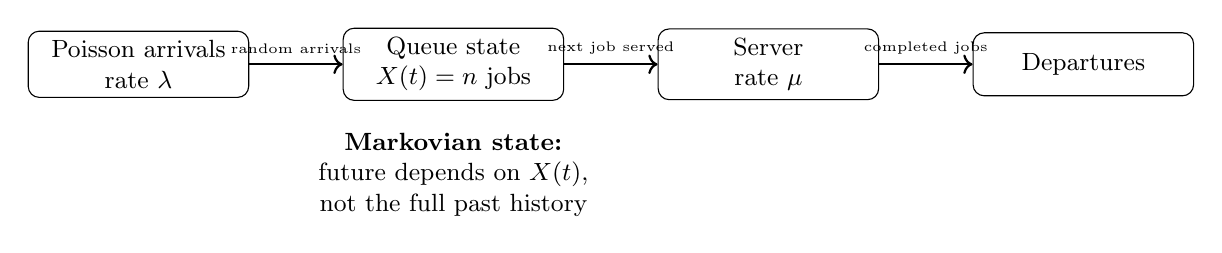
\begin{tikzpicture}[
    font=\small,
    box/.style={
        rectangle,
        rounded corners,
        draw,
        align=center,
        minimum width=2.8cm,
        minimum height=0.8cm
    },
    arrow/.style={->, thick}
]

\node[box] (arrivals) at (0,0) {Poisson arrivals\\rate $\lambda$};
\node[box] (queue) at (4,0) {Queue state\\$X(t)=n$ jobs};
\node[box] (server) at (8,0) {Server\\rate $\mu$};
\node[box] (departures) at (12,0) {Departures};

\draw[arrow] (arrivals) -- node[above] {\tiny random arrivals} (queue);
\draw[arrow] (queue) -- node[above] {\tiny next job served} (server);
\draw[arrow] (server) -- node[above] {\tiny completed jobs} (departures);

\node[align=center] at (4,-1.4) {
    \textbf{Markovian state:}\\
    future depends on $X(t)$,\\
    not the full past history
};

\end{tikzpicture}
\end{center}

\vspace{0.2cm}

\begin{alertblock}{Simple summary}
Poisson tells us how jobs arrive. Markovian tells us the current state is enough to reason about what happens next.
\end{alertblock}

\end{frame}



\begin{frame}{Queueing Theory Translated into Sales/Customer Language}
\scriptsize

\begin{tabular}{p{3.0cm} p{7.8cm}}
\toprule
\textbf{Queueing Theory Term} & \textbf{Sales / Customer Language} \\
\midrule
\textbf{Arrival rate} & incoming calls, requests, packets, tickets \\
\textbf{Service rate} & how fast agents, servers, or links process work \\
\textbf{Server} & agent, CPU worker, trunk channel, encoder, link \\
\textbf{Queue length} & backlog, hold queue, pending requests \\
\textbf{Waiting time} & hold time, delay, latency \\
\textbf{Utilization} & saturation, busyness, capacity usage \\
\textbf{Stability} & can the system keep up? \\
\textbf{Burstiness} & spikes, surges, peak traffic \\
\textbf{Tail latency} & worst-user experience \\
\textbf{Blocking} & failed calls, rejected requests, busy signals \\
\textbf{Abandonment} & callers hang up, users retry or leave \\
\textbf{Priority queue} & QoS, VIP routing, emergency priority \\
\textbf{Finite buffer} & queue limit, max pending, dropped work \\
\textbf{Drop policy} & fail fast, drop stale, reject overflow \\
\bottomrule
\end{tabular}

\vspace{0.15cm}

\begin{alertblock}{Why this matters}
Queueing theory gives you a technical lens for explaining customer pain in practical business terms: congestion, delay, backlog, failed calls, poor user experience, and capacity limits.
\end{alertblock}

\end{frame}
















\section{5G}

\begin{frame}
    \centering
    \vfill

    {\Huge \textbf{LTE/5G/Wireless}}

    \vspace{0.4cm}

    {\Large Lets get into it}

    \vfill
\end{frame}



\begin{frame}{LTE/5G/Wireless Terms: Core Architecture}
\tiny
\begin{tabular}{p{2.0cm} p{3.4cm} p{6.7cm}}
\toprule
\textbf{Term} & \textbf{Meaning} & \textbf{Why it matters} \\
\midrule
\textbf{UE} & User Equipment & Phone, modem, IoT device, router, or radio endpoint connected to the network. \\
\textbf{RAN} & Radio Access Network & Wireless part of the network connecting UEs to the carrier core. \\
\textbf{eNodeB} & LTE base station & LTE radio node that serves UEs over the air interface. \\
\textbf{gNodeB} & 5G base station & 5G NR radio node that serves UEs over the air interface. \\
\textbf{EPC} & Evolved Packet Core & LTE core network for mobility, authentication, routing, and internet access. \\
\textbf{5GC} & 5G Core & 5G service-based core architecture. \\
\textbf{MME} & Mobility Management Entity & LTE control-plane function for attach, mobility, and bearer management. \\
\textbf{AMF} & Access and Mobility Management Function & 5G control-plane function for registration, connection, and mobility management. \\
\textbf{SMF} & Session Management Function & 5G function that manages PDU sessions and user-plane routing. \\
\textbf{UPF} & User Plane Function & 5G user-plane anchor that forwards user traffic. \\
\textbf{SA} & Standalone 5G & 5G NR connected to 5G Core. \\
\textbf{NSA} & Non-Standalone 5G & 5G NR assisted by LTE core/control plane. \\
\bottomrule
\end{tabular}

\vspace{0.15cm}
\begin{block}{Mental model}
The UE talks to the RAN over radio. The RAN connects into the core. The core handles identity, mobility, sessions, routing, and policy.
\end{block}
\end{frame}




\begin{frame}{LTE/5G/Wireless Terms: Radio and Spectrum}
\tiny
\begin{tabular}{p{2.0cm} p{3.4cm} p{6.7cm}}
\toprule
\textbf{Term} & \textbf{Meaning} & \textbf{Why it matters} \\
\midrule
\textbf{RF} & Radio Frequency & Electromagnetic spectrum used for wireless communication. \\
\textbf{Band} & Frequency allocation & Defines what frequencies a carrier/device can use. \\
\textbf{Channel} & Slice of spectrum & The actual frequency resource used to transmit data. \\
\textbf{Bandwidth} & Width of channel & More bandwidth usually means more potential throughput. \\
\textbf{Subcarrier} & Small OFDM frequency bin & LTE/5G divide wide channels into many narrow subcarriers. \\
\textbf{OFDM} & Orthogonal Frequency-Division Multiplexing & Modulation framework used by LTE downlink and 5G NR. \\
\textbf{OFDMA} & OFDM Multiple Access & Lets users share subcarriers/time resources. \\
\textbf{TDD} & Time Division Duplex & Uplink/downlink share same frequency but different time slots. \\
\textbf{FDD} & Frequency Division Duplex & Uplink/downlink use separate frequency bands. \\
\textbf{FR1} & 5G sub-7 GHz range & Better coverage and penetration. \\
\textbf{FR2} & 5G mmWave range & High bandwidth, shorter range, weaker penetration. \\
\textbf{mmWave} & Millimeter wave & Very high-frequency 5G spectrum with high capacity but coverage challenges. \\
\bottomrule
\end{tabular}

\vspace{0.15cm}
\begin{block}{Mental model}
Wireless capacity depends on spectrum, bandwidth, signal quality, modulation, antenna design, and how radio resources are scheduled.
\end{block}
\end{frame}


\begin{frame}{LTE/5G/Wireless Terms: Signal Quality}
\tiny
\begin{tabular}{p{2.0cm} p{3.4cm} p{6.7cm}}
\toprule
\textbf{Term} & \textbf{Meaning} & \textbf{Why it matters} \\
\midrule
\textbf{RSSI} & Received Signal Strength Indicator & General received power measurement. \\
\textbf{RSRP} & Reference Signal Received Power & LTE/5G signal strength metric for reference signals. \\
\textbf{RSRQ} & Reference Signal Received Quality & Signal quality metric that reflects load/interference. \\
\textbf{SINR} & Signal-to-Interference-plus-Noise Ratio & Key quality metric; higher SINR supports better modulation/coding. \\
\textbf{SNR} & Signal-to-Noise Ratio & Signal strength relative to noise. \\
\textbf{CQI} & Channel Quality Indicator & UE feedback used by base station for scheduling and modulation. \\
\textbf{MCS} & Modulation and Coding Scheme & Determines how aggressively bits are packed onto the radio channel. \\
\textbf{BLER} & Block Error Rate & Fraction of radio transport blocks received incorrectly. \\
\textbf{HARQ} & Hybrid Automatic Repeat Request & Fast retransmission/error recovery mechanism. \\
\textbf{Path loss} & Signal attenuation over distance & More path loss means weaker received signal. \\
\textbf{Fading} & Rapid signal variation & Caused by mobility, multipath, obstruction, and interference. \\
\textbf{Interference} & Unwanted energy from other transmissions & Reduces usable signal quality and throughput. \\
\bottomrule
\end{tabular}

\vspace{0.15cm}
\begin{block}{Mental model}
Wireless is not just bars. Throughput and reliability depend on signal strength, interference, fading, coding, retransmissions, and scheduling.
\end{block}
\end{frame}



\begin{frame}{LTE/5G/Wireless Terms: Performance and QoS}
\tiny
\begin{tabular}{p{2.0cm} p{3.4cm} p{6.7cm}}
\toprule
\textbf{Term} & \textbf{Meaning} & \textbf{Why it matters} \\
\midrule
\textbf{Throughput} & Delivered data rate & What the application actually receives. \\
\textbf{Latency} & Time delay & Critical for voice, gaming, video, control, and teleoperation. \\
\textbf{Jitter} & Delay variation & Critical for RTP, VoIP, video, and real-time control. \\
\textbf{Packet loss} & Missing packets & Causes media artifacts, retransmissions, or application failure. \\
\textbf{QoS} & Quality of Service & Traffic treatment based on priority and service requirements. \\
\textbf{QCI} & QoS Class Identifier & LTE QoS class for bearers. \\
\textbf{5QI} & 5G QoS Identifier & 5G QoS class for flows. \\
\textbf{GBR} & Guaranteed Bit Rate & QoS flow/bearer with guaranteed bandwidth treatment. \\
\textbf{Non-GBR} & Non-Guaranteed Bit Rate & Best-effort or elastic traffic treatment. \\
\textbf{Bearer} & LTE logical traffic pipe & Carries user traffic with specific QoS characteristics. \\
\textbf{PDU Session} & 5G user data session & 5G session connecting UE to data network. \\
\textbf{Network slicing} & Logical network partitioning & 5G feature for separate service profiles over shared infrastructure. \\
\bottomrule
\end{tabular}

\vspace{0.15cm}
\begin{block}{Mental model}
Real-time wireless performance is shaped by radio quality, scheduler decisions, QoS class, congestion, retransmissions, and core-network path.
\end{block}
\end{frame}


\begin{frame}{Queueing Theory Meets Wireless}
\tiny

\begin{tabular}{p{2.4cm} p{4.0cm} p{5.8cm}}
\toprule
\textbf{Queueing Concept} & \textbf{Wireless Equivalent} & \textbf{Why it matters} \\
\midrule
\textbf{Arrival rate} $\lambda$ & Packets arriving from apps/UEs & Voice, video, telemetry, and bulk data compete for service. \\
\textbf{Service rate} $\mu$ & How fast the radio link can transmit & Changes with SINR, MCS, bandwidth, scheduling, and mobility. \\
\textbf{Server} & Radio resource, scheduler, base station, channel & Wireless capacity is shared across users and time-frequency resources. \\
\textbf{Queue length} & Buffered packets waiting for uplink/downlink grants & More backlog usually means more latency. \\
\textbf{Waiting time} & Time waiting before transmission & Drives latency and jitter for real-time traffic. \\
\textbf{Utilization} $\rho$ & How loaded the cell/link/scheduler is & As load approaches capacity, delay can grow sharply. \\
\textbf{Burstiness} & Traffic spikes or channel quality drops & Queues can build even if average load looks acceptable. \\
\textbf{Tail latency} & p95/p99 wireless delay & Critical for VoIP, teleoperation, gaming, and control loops. \\
\bottomrule
\end{tabular}

\vspace{0.15cm}

\begin{alertblock}{Mental model}
Wireless latency is often queueing delay plus radio uncertainty: packets wait for capacity, grants, retransmissions, and a good enough channel.
\end{alertblock}

\end{frame}


\begin{frame}{Why Wireless Service Rate Is Not Constant}
\tiny

\begin{block}{Core idea}
In wired systems, link capacity is often relatively stable. In wireless systems, the effective service rate changes over time.
\end{block}

\vspace{0.15cm}

\begin{columns}[T]
\column{0.48\textwidth}

\textbf{Service rate depends on}

\begin{itemize}
    \item Signal quality: \texttt{SINR}, \texttt{RSRP}, \texttt{RSRQ}
    \item Modulation and coding: \texttt{MCS}
    \item Available bandwidth
    \item Scheduler decisions
    \item Number of active users
    \item Mobility and handovers
    \item Interference and fading
    \item HARQ retransmissions
\end{itemize}

\column{0.48\textwidth}

\textbf{Queueing consequence}

\begin{itemize}
    \item Good channel: high $\mu$, queue drains
    \item Bad channel: low $\mu$, queue builds
    \item Congested cell: users wait longer for resources
    \item Retransmissions consume future capacity
    \item Bursts create p95/p99 delay spikes
\end{itemize}

\end{columns}

\vspace{0.15cm}

\begin{alertblock}{Engineering translation}
In wireless, $\mu$ is not a fixed number. It is a moving target controlled by channel quality, scheduling, coding, load, and retransmissions.
\end{alertblock}

\end{frame}



\begin{frame}{Wireless Scheduling as Queue Management}
\tiny

\begin{block}{Core idea}
The base station scheduler decides which users get radio resources, when they get them, and how much they get.
\end{block}

\vspace{0.15cm}

\begin{tabular}{p{2.6cm} p{4.0cm} p{5.5cm}}
\toprule
\textbf{Scheduler Question} & \textbf{Queueing View} & \textbf{Wireless Impact} \\
\midrule
Who transmits next? & Service discipline & Determines fairness, priority, and delay. \\
How much capacity? & Service quantum & Controls how many queued bits can drain. \\
Which traffic class? & Priority queueing & Real-time traffic may need priority over bulk data. \\
Which UE has good channel? & Opportunistic service & Good-channel users can be served efficiently. \\
Which UE is waiting too long? & Delay-aware scheduling & Prevents starvation and tail-latency spikes. \\
What gets retransmitted? & Re-service after failure & HARQ/ARQ can protect reliability but adds delay. \\
\bottomrule
\end{tabular}

\vspace{0.15cm}

\begin{alertblock}{Mental model}
A wireless scheduler is not just allocating bandwidth. It is constantly managing queues under changing channel conditions.
\end{alertblock}

\end{frame}


\begin{frame}{Wireless QoS Through a Queueing Lens}
\tiny

\begin{block}{Core idea}
QoS classes are basically promises about how different queues should be treated under contention.
\end{block}

\vspace{0.15cm}

\begin{tabular}{p{2.4cm} p{4.0cm} p{5.8cm}}
\toprule
\textbf{Traffic Type} & \textbf{Queueing Need} & \textbf{Wireless Concern} \\
\midrule
\textbf{VoIP} & Low delay, low jitter, small packets & Needs priority and stable scheduling; late packets are useless. \\
\textbf{Video} & High throughput, bounded delay & Buffers can smooth jitter but increase latency. \\
\textbf{Teleoperation} & Low tail latency, high freshness & Stale frames/control data may be worse than dropped data. \\
\textbf{Telemetry} & Reliability and timely updates & Bursts can queue behind less important traffic. \\
\textbf{Bulk data} & Throughput over latency & Can fill buffers and hurt real-time traffic. \\
\textbf{Emergency traffic} & Priority and survivability & Needs preferential access under congestion. \\
\bottomrule
\end{tabular}

\vspace{0.15cm}

\begin{alertblock}{Engineering takeaway}
QoS is queue policy: which traffic waits, which traffic gets served first, and which traffic is allowed to build backlog.
\end{alertblock}

\end{frame}


\begin{frame}{Wireless Retransmissions: Reliability vs. Delay}
\tiny

\begin{block}{Core idea}
Wireless links use retransmissions to recover from errors, but retransmissions consume time and capacity.
\end{block}

\vspace{0.15cm}

\begin{columns}[T]
\column{0.48\textwidth}

\textbf{Reliability benefit}

\begin{itemize}
    \item Bad radio blocks can be resent
    \item Packet loss decreases
    \item Throughput may improve under moderate errors
    \item Applications see fewer missing packets
\end{itemize}

\vspace{0.1cm}

\textbf{Wireless mechanisms}

\begin{itemize}
    \item HARQ
    \item ARQ
    \item coding redundancy
    \item link adaptation
\end{itemize}

\column{0.48\textwidth}

\textbf{Queueing cost}

\begin{itemize}
    \item Retransmitted work competes with new work
    \item Queue service capacity is consumed by retries
    \item Waiting time increases
    \item Jitter increases
    \item Tail latency can spike
\end{itemize}

\vspace{0.1cm}

\textbf{Real-time tradeoff}

\begin{itemize}
    \item For files: late is better than missing
    \item For live media: late may be useless
\end{itemize}

\end{columns}

\vspace{0.15cm}

\begin{alertblock}{Mental model}
Wireless reliability mechanisms reduce loss, but they can increase delay because the system spends service time repairing old transmissions.
\end{alertblock}

\end{frame}




\begin{frame}{Queueing Theory Explains Wireless Pain}
\scriptsize

\begin{tabular}{p{3.0cm} p{4.0cm} p{5.0cm}}
\toprule
\textbf{Customer Symptom} & \textbf{Queueing Diagnosis} & \textbf{Wireless Cause} \\
\midrule
Voice gets choppy & Jitter and packet delay variation & Congestion, retransmissions, weak SINR, scheduler delay \\
Video lags behind reality & Frame age / buffer buildup & Pipeline or radio queue preserving stale frames \\
Works until peak hours & Utilization approaching capacity & Too many users sharing limited cell resources \\
Good speed test, bad calls & Average throughput hides tail latency & Real-time packets wait behind bursts or bulk traffic \\
Random delay spikes & Variable service rate & Fading, interference, handover, HARQ retries \\
Drone/control feels delayed & Tail latency and stale state & Queues form during bad channel periods or congestion \\
Packets arrive in bursts & Service opportunities are uneven & Scheduling grants and changing channel quality \\
\bottomrule
\end{tabular}

\vspace{0.15cm}

\begin{alertblock}{One-sentence insight}
Wireless problems are often not just “coverage” problems; they are dynamic queueing problems caused by shared capacity, variable service rate, retransmissions, and contention.
\end{alertblock}

\end{frame}






















\section{RF/MANET}

\begin{frame}
    \centering
    \vfill

    {\Huge \textbf{RF/MANET}}

    \vspace{0.4cm}

    {\Large Lets get into it}

    \vfill
\end{frame}


\begin{frame}{RF Terms: Core Radio Concepts}
\tiny
\begin{tabular}{p{2.0cm} p{3.4cm} p{6.7cm}}
\toprule
\textbf{Term} & \textbf{Meaning} & \textbf{Why it matters} \\
\midrule
\textbf{RF} & Radio Frequency & Electromagnetic signals used for wireless communication. \\
\textbf{Frequency} & Cycles per second & Determines wavelength, propagation, antenna size, and band usage. \\
\textbf{Wavelength} & Physical length of one wave cycle & Lower frequencies have longer wavelengths and often better penetration. \\
\textbf{Bandwidth} & Width of frequency range & More bandwidth usually supports more data capacity. \\
\textbf{Channel} & Assigned slice of spectrum & Radios communicate over specific channels/frequencies. \\
\textbf{Modulation} & Encoding data onto a carrier wave & Determines how bits are represented over RF. \\
\textbf{Carrier} & Base RF signal & Signal that gets modulated to carry information. \\
\textbf{Noise floor} & Background RF noise level & Sets the baseline that signals must rise above. \\
\textbf{Interference} & Unwanted RF energy & Reduces signal quality and can cause packet loss or lower throughput. \\
\textbf{Spectrum} & Range of RF frequencies & Wireless systems compete for limited spectrum resources. \\
\textbf{ISM band} & Industrial, Scientific, Medical band & Unlicensed bands commonly used by Wi-Fi, Bluetooth, telemetry, and radios. \\
\bottomrule
\end{tabular}

\vspace{0.15cm}
\begin{block}{Mental model}
RF communication is about pushing useful signal through noise, interference, distance, obstacles, and limited spectrum.
\end{block}
\end{frame}




\begin{frame}{RF Terms: Power, Gain, and Link Budget}
\tiny
\begin{tabular}{p{2.0cm} p{3.4cm} p{6.7cm}}
\toprule
\textbf{Term} & \textbf{Meaning} & \textbf{Why it matters} \\
\midrule
\textbf{dB} & Decibel & Logarithmic ratio used for gains and losses. \\
\textbf{dBm} & dB relative to 1 milliwatt & Common unit for transmit power and received signal strength. \\
\textbf{Tx Power} & Transmit power & More power can improve range but is limited by regulation, battery, and interference. \\
\textbf{Rx Sensitivity} & Minimum usable receive power & Lower sensitivity threshold means the receiver can decode weaker signals. \\
\textbf{Antenna Gain} & Directional concentration of energy & Increases effective signal in favored directions. \\
\textbf{EIRP} & Effective Isotropic Radiated Power & Total radiated power after transmitter power, cable loss, and antenna gain. \\
\textbf{Cable Loss} & Signal loss in feedline/connectors & Reduces power reaching antenna or receiver. \\
\textbf{Path Loss} & Signal loss over distance & Major factor in range and link reliability. \\
\textbf{Link Budget} & Accounting of all gains/losses & Predicts whether a wireless link should close. \\
\textbf{Fade Margin} & Extra signal above required minimum & More margin means better resilience to fading and interference. \\
\textbf{SNR} & Signal-to-Noise Ratio & Higher SNR generally enables better data rates and reliability. \\
\textbf{SINR} & Signal-to-Interference-plus-Noise Ratio & More realistic metric when other transmitters are present. \\
\bottomrule
\end{tabular}

\vspace{0.15cm}
\begin{block}{Mental model}
A link works when received signal power stays far enough above noise, interference, and receiver sensitivity.
\end{block}
\end{frame}


\begin{frame}{RF Terms: Power, Gain, and Link Budget}
\tiny
\begin{tabular}{p{2.0cm} p{3.4cm} p{6.7cm}}
\toprule
\textbf{Term} & \textbf{Meaning} & \textbf{Why it matters} \\
\midrule
\textbf{dB} & Decibel & Logarithmic ratio used for gains and losses. \\
\textbf{dBm} & dB relative to 1 milliwatt & Common unit for transmit power and received signal strength. \\
\textbf{Tx Power} & Transmit power & More power can improve range but is limited by regulation, battery, and interference. \\
\textbf{Rx Sensitivity} & Minimum usable receive power & Lower sensitivity threshold means the receiver can decode weaker signals. \\
\textbf{Antenna Gain} & Directional concentration of energy & Increases effective signal in favored directions. \\
\textbf{EIRP} & Effective Isotropic Radiated Power & Total radiated power after transmitter power, cable loss, and antenna gain. \\
\textbf{Cable Loss} & Signal loss in feedline/connectors & Reduces power reaching antenna or receiver. \\
\textbf{Path Loss} & Signal loss over distance & Major factor in range and link reliability. \\
\textbf{Link Budget} & Accounting of all gains/losses & Predicts whether a wireless link should close. \\
\textbf{Fade Margin} & Extra signal above required minimum & More margin means better resilience to fading and interference. \\
\textbf{SNR} & Signal-to-Noise Ratio & Higher SNR generally enables better data rates and reliability. \\
\textbf{SINR} & Signal-to-Interference-plus-Noise Ratio & More realistic metric when other transmitters are present. \\
\bottomrule
\end{tabular}

\vspace{0.15cm}
\begin{block}{Mental model}
A link works when received signal power stays far enough above noise, interference, and receiver sensitivity.
\end{block}
\end{frame}


\begin{frame}{RF Terms: Antennas and Propagation}
\scriptsize
\begin{tabular}{p{2.0cm} p{3.4cm} p{6.7cm}}
\toprule
\textbf{Term} & \textbf{Meaning} & \textbf{Why it matters} \\
\midrule
\textbf{Omni Antenna} & Radiates broadly around itself & Useful for mobile users and general coverage. \\
\textbf{Directional Antenna} & Focuses energy in a direction & Improves range/SNR but requires aiming. \\
\textbf{Polarization} & Orientation of electric field & Mismatched polarization causes signal loss. \\
\textbf{LOS} & Line of Sight & Clear path between radios; usually best for RF links. \\
\textbf{NLOS} & Non-Line of Sight & Obstructed path; more fading, loss, and multipath. \\
\textbf{Multipath} & Reflections create multiple signal paths & Can cause fading, delay spread, and interference with itself. \\
\textbf{Fresnel Zone} & Elliptical RF clearance region & Even with visual LOS, obstruction in this zone can weaken the link. \\
\textbf{Reflection} & Signal bounces off surfaces & Can help or hurt depending on phase/path. \\
\textbf{Diffraction} & Signal bends around edges & Helps lower-frequency signals reach obstructed areas. \\
\textbf{Absorption} & Energy lost in materials & Trees, buildings, rain, and terrain can attenuate RF. \\
\textbf{Doppler Shift} & Frequency shift due to motion & Important for fast-moving nodes, UAVs, and mobile networks. \\
\bottomrule
\end{tabular}

\vspace{0.15cm}
\begin{block}{Mental model}
Wireless range is not just distance. It is antenna pattern, path clearance, terrain, reflections, polarization, and mobility.
\end{block}
\end{frame}

\begin{frame}{RF Terms: Modulation, Coding, and Throughput}
\tiny
\begin{tabular}{p{2.0cm} p{3.4cm} p{6.7cm}}
\toprule
\textbf{Term} & \textbf{Meaning} & \textbf{Why it matters} \\
\midrule
\textbf{BPSK} & Binary Phase Shift Keying & Robust, low data rate modulation. \\
\textbf{QPSK} & Quadrature Phase Shift Keying & Moderate robustness and spectral efficiency. \\
\textbf{QAM} & Quadrature Amplitude Modulation & Higher-order QAM carries more bits but needs better SNR. \\
\textbf{MCS} & Modulation and Coding Scheme & Selects modulation and error coding based on channel quality. \\
\textbf{FEC} & Forward Error Correction & Adds redundancy so receiver can correct errors. \\
\textbf{Coding Rate} & Payload fraction after error coding & Higher coding rate means less redundancy but more sensitivity to errors. \\
\textbf{Symbol Rate} & Symbols transmitted per second & Related to bandwidth and data rate. \\
\textbf{Spectral Efficiency} & Bits/s/Hz & Measures how efficiently bandwidth carries data. \\
\textbf{BER} & Bit Error Rate & Fraction of bits received incorrectly. \\
\textbf{PER} & Packet Error Rate & Fraction of packets lost or corrupted. \\
\textbf{Adaptive Modulation} & Change MCS with channel quality & Trades throughput for reliability as RF conditions change. \\
\bottomrule
\end{tabular}

\vspace{0.15cm}
\begin{block}{Mental model}
Higher data rates require better RF conditions. When the channel degrades, the system usually lowers modulation/coding to survive.
\end{block}
\end{frame}


\begin{frame}{MANET Terms: Core Concepts}
\tiny
\begin{tabular}{p{2.0cm} p{3.4cm} p{6.7cm}}
\toprule
\textbf{Term} & \textbf{Meaning} & \textbf{Why it matters} \\
\midrule
\textbf{MANET} & Mobile Ad Hoc Network & Self-forming wireless network without fixed infrastructure. \\
\textbf{Node} & Radio/device in the network & Each node may send, receive, and forward traffic. \\
\textbf{Ad Hoc} & Infrastructureless networking & Nodes organize dynamically instead of relying on towers/APs. \\
\textbf{Mesh Network} & Multi-node connected network & Traffic can route through neighboring nodes. \\
\textbf{Multi-hop} & Packets traverse multiple radios & Extends range but adds delay, contention, and failure points. \\
\textbf{Neighbor} & Directly reachable node & Routing depends on discovering and maintaining neighbors. \\
\textbf{Topology} & Network connectivity graph & Changes as nodes move, links fade, or radios fail. \\
\textbf{Self-healing} & Re-routing around failures & Critical for tactical and mobile environments. \\
\textbf{Mobility} & Node movement & Causes changing link quality, route churn, and handoff-like behavior. \\
\textbf{Backhaul} & Link from edge mesh to wider network & Connects MANET to command center, internet, or enterprise network. \\
\textbf{Gateway Node} & Bridge to another network & Often becomes a bottleneck or critical dependency. \\
\bottomrule
\end{tabular}

\vspace{0.15cm}
\begin{block}{Mental model}
A MANET is a moving graph of radios where links appear, degrade, disappear, and re-route dynamically.
\end{block}
\end{frame}



\begin{frame}{MANET Terms: Routing and Control}
\tiny
\begin{tabular}{p{2.0cm} p{3.4cm} p{6.7cm}}
\toprule
\textbf{Term} & \textbf{Meaning} & \textbf{Why it matters} \\
\midrule
\textbf{Routing Protocol} & Chooses packet paths & Determines how traffic moves through the mesh. \\
\textbf{Proactive Routing} & Maintains routes continuously & Lower route discovery delay but more control overhead. \\
\textbf{Reactive Routing} & Finds routes on demand & Lower idle overhead but route discovery can add delay. \\
\textbf{Hybrid Routing} & Mix of proactive/reactive & Balances overhead and responsiveness. \\
\textbf{Route Discovery} & Process of finding path & Adds latency when paths are unknown or broken. \\
\textbf{Route Maintenance} & Keeping paths valid & Needed under mobility and fading. \\
\textbf{Hop Count} & Number of links in path & More hops usually means more delay and more contention. \\
\textbf{Metric} & Cost used for route choice & Could include hop count, link quality, ETX, latency, or bandwidth. \\
\textbf{ETX} & Expected Transmission Count & Estimates how many transmissions are needed for successful delivery. \\
\textbf{Control Overhead} & Routing/management traffic & Consumes airtime that could carry user data. \\
\textbf{Flooding} & Broadcast propagation method & Useful for discovery but can overload the network. \\
\textbf{Convergence} & Time to settle on valid routes & Slow convergence creates packet loss and delay spikes. \\
\bottomrule
\end{tabular}

\vspace{0.15cm}
\begin{block}{Mental model}
MANET routing is a constant tradeoff between route freshness, overhead, stability, and latency.
\end{block}
\end{frame}



\begin{frame}{MANET Terms: Performance and Reliability}
\tiny
\begin{tabular}{p{2.0cm} p{3.4cm} p{6.7cm}}
\toprule
\textbf{Term} & \textbf{Meaning} & \textbf{Why it matters} \\
\midrule
\textbf{Throughput} & Delivered data rate & Drops as links degrade or hops increase. \\
\textbf{Latency} & End-to-end delay & Accumulates across queues, hops, retransmissions, and route changes. \\
\textbf{Jitter} & Delay variation & Hurts voice, video, and control traffic. \\
\textbf{PDR} & Packet Delivery Ratio & Fraction of packets successfully delivered. \\
\textbf{Goodput} & Useful application throughput & Excludes retransmissions and overhead. \\
\textbf{Airtime} & Shared RF transmission time & The true scarce resource in wireless mesh. \\
\textbf{Contention} & Nodes competing for channel access & More contention increases delay and collisions. \\
\textbf{Hidden Node} & Nodes cannot hear each other but collide at receiver & Classic wireless problem that reduces reliability. \\
\textbf{Retransmission} & Resending failed packets & Improves delivery but increases delay and airtime use. \\
\textbf{Route Flap} & Frequent route changes & Causes instability, loss, and jitter. \\
\textbf{Bottleneck Link} & Weakest path segment & Limits end-to-end throughput and drives queueing. \\
\textbf{Partition} & Network splits into disconnected groups & Some nodes become unreachable. \\
\bottomrule
\end{tabular}

\vspace{0.15cm}
\begin{block}{Mental model}
In a MANET, performance is constrained by shared airtime, hop count, link quality, mobility, and routing stability.
\end{block}
\end{frame}


\begin{frame}{RF/MANET Terms: Tactical Networking Lens}
\tiny
\begin{tabular}{p{2.0cm} p{3.4cm} p{6.7cm}}
\toprule
\textbf{Term} & \textbf{Meaning} & \textbf{Why it matters} \\
\midrule
\textbf{LOS Link} & Direct unobstructed RF path & Usually stronger and higher capacity. \\
\textbf{Relay Node} & Node forwarding traffic for others & Extends range but adds hop delay and airtime use. \\
\textbf{Edge Node} & Node at network boundary & Often has weaker connectivity and more fragile routes. \\
\textbf{Mobility Pattern} & How nodes move & Determines route churn and link stability. \\
\textbf{Network Density} & Number of nodes in area & Too sparse causes partitions; too dense causes contention. \\
\textbf{Jamming} & Intentional RF interference & Degrades or denies communication. \\
\textbf{LPI/LPD} & Low Probability of Intercept/Detection & Techniques to reduce detectability by adversaries. \\
\textbf{EMCON} & Emissions Control & Controls transmissions to reduce signature or interference. \\
\textbf{SATCOM} & Satellite Communications & Can provide beyond-line-of-sight backhaul. \\
\textbf{BLOS} & Beyond Line of Sight & Communication beyond direct RF horizon, often via relay or satellite. \\
\textbf{QoS} & Quality of Service & Prioritizes critical traffic such as voice/control over bulk data. \\
\textbf{C2} & Command and Control & Mission-critical traffic requiring resilience and timeliness. \\
\bottomrule
\end{tabular}

\vspace{0.15cm}
\begin{block}{Mental model}
Tactical wireless is not just connectivity. It is range, survivability, mobility, detectability, priority, and mission-critical timing.
\end{block}
\end{frame}





\section{Security}

\begin{frame}
    \centering
    \vfill

    {\Huge \textbf{Cybersecurity}}

    \vspace{0.4cm}

    {\Large Lets get into it}

    \vfill
\end{frame}


\begin{frame}{Cybersecurity Terms: Real-Time Communications Threat Model}
\tiny
\begin{tabular}{p{2.2cm} p{3.5cm} p{6.5cm}}
\toprule
\textbf{Term} & \textbf{Meaning} & \textbf{Why it matters for RTC} \\
\midrule
\textbf{CIA Triad} & Confidentiality, Integrity, Availability & RTC must keep media private, prevent tampering, and remain reachable. \\
\textbf{Threat Model} & Structured view of risks & Defines who can attack, what they target, and what defenses matter. \\
\textbf{Attack Surface} & Exposed entry points & SIP ports, RTP ports, APIs, radios, VPNs, web clients, and management interfaces. \\
\textbf{Adversary} & Attacker or hostile actor & Could be spammer, fraudster, insider, RF jammer, or nation-state actor. \\
\textbf{Asset} & Thing being protected & Calls, media streams, credentials, keys, location, availability, routing policy. \\
\textbf{Trust Boundary} & Boundary between security domains & Example: LAN to internet, UE to RAN, enterprise to SIP carrier, MANET to backhaul. \\
\textbf{Control Plane} & Signaling/management path & SIP, routing, authentication, registration, scheduling, and session control. \\
\textbf{Data Plane} & User traffic/media path & RTP/SRTP packets, video frames, voice packets, telemetry, C2 traffic. \\
\textbf{Blast Radius} & Scope of damage & Measures how far compromise or outage spreads. \\
\bottomrule
\end{tabular}

\vspace{0.15cm}
\begin{block}{Mental model}
Real-time communications security is not just encryption. It is protecting signaling, media, identity, availability, routing, and timing.
\end{block}
\end{frame}


\begin{frame}{Cybersecurity Terms: Identity and Access}
\tiny
\begin{tabular}{p{2.2cm} p{3.5cm} p{6.5cm}}
\toprule
\textbf{Term} & \textbf{Meaning} & \textbf{Why it matters for RTC} \\
\midrule
\textbf{Authentication} & Proving identity & Verifies users, devices, phones, radios, SIP peers, and APIs. \\
\textbf{Authorization} & Permission to act & Determines who can place calls, access trunks, join meetings, or manage devices. \\
\textbf{Accounting} & Logging usage/activity & Tracks calls, registrations, admin actions, and suspicious behavior. \\
\textbf{AAA} & AuthN, AuthZ, Accounting & Core framework for access control and operational accountability. \\
\textbf{MFA} & Multi-Factor Authentication & Reduces risk of stolen-password compromise. \\
\textbf{RBAC} & Role-Based Access Control & Gives users permissions based on role, such as admin, operator, analyst. \\
\textbf{Least Privilege} & Minimum needed access & Limits damage if an account, device, or service is compromised. \\
\textbf{Zero Trust} & Never trust by location alone & Every device/session must be verified, even inside the network. \\
\textbf{Credential Stuffing} & Reuse of stolen passwords & Common threat against cloud voice/admin portals. \\
\textbf{Brute Force} & Guessing credentials repeatedly & Common against SIP registrations and exposed admin interfaces. \\
\bottomrule
\end{tabular}

\vspace{0.15cm}
\begin{block}{Mental model}
If an attacker can impersonate a user, phone, SIP trunk, radio node, or admin, they can redirect traffic, steal service, or disrupt communications.
\end{block}
\end{frame}


\begin{frame}{Cybersecurity Terms: Encryption and Keying}
\tiny
\begin{tabular}{p{2.2cm} p{3.5cm} p{6.5cm}}
\toprule
\textbf{Term} & \textbf{Meaning} & \textbf{Why it matters for RTC} \\
\midrule
\textbf{Encryption} & Converts plaintext to ciphertext & Protects SIP signaling, media, VPN traffic, and management traffic. \\
\textbf{Integrity} & Detects unauthorized modification & Prevents tampering with signaling, packets, updates, and commands. \\
\textbf{Authentication Tag} & Cryptographic integrity check & Lets receiver verify packet/message authenticity. \\
\textbf{Key Exchange} & Establishing shared keys & Needed before secure communication can begin. \\
\textbf{Symmetric Key} & Same key encrypts/decrypts & Efficient for media streams like SRTP. \\
\textbf{Asymmetric Key} & Public/private key pair & Used in TLS certificates and identity validation. \\
\textbf{PFS} & Perfect Forward Secrecy & Past traffic stays protected even if long-term key is later compromised. \\
\textbf{PKI} & Public Key Infrastructure & Certificate trust system used by TLS and device identity. \\
\textbf{Certificate} & Signed identity credential & Proves server/client identity in TLS or mTLS. \\
\textbf{Key Rotation} & Replacing keys over time & Limits exposure from leaked or old keys. \\
\bottomrule
\end{tabular}

\vspace{0.15cm}
\begin{block}{Mental model}
Encryption protects confidentiality, but real security also requires identity, integrity, correct key management, and replay protection.
\end{block}
\end{frame}



\begin{frame}{Cybersecurity Terms: SIP/TLS/SRTP Security}
\tiny
\begin{tabular}{p{2.2cm} p{3.5cm} p{6.5cm}}
\toprule
\textbf{Term} & \textbf{Meaning} & \textbf{Why it matters for RTC} \\
\midrule
\textbf{SIP over TLS} & SIP carried inside TLS & Protects signaling messages, headers, and SDP in transit. \\
\textbf{SRTP} & Secure RTP & Encrypts and authenticates real-time media packets. \\
\textbf{SIPS} & Secure SIP URI scheme & Indicates SIP should use secure transport. \\
\textbf{SDES} & SRTP keys in SDP & Simple SRTP keying method; depends heavily on protecting SIP/SDP. \\
\textbf{DTLS-SRTP} & DTLS establishes SRTP keys & Common WebRTC media-security model. \\
\textbf{mTLS} & Mutual TLS & Both endpoints authenticate with certificates. \\
\textbf{Digest Auth} & SIP challenge-response auth & Common SIP auth method that avoids sending raw password. \\
\textbf{Replay Protection} & Blocks reused packets & Important for SRTP and command/control traffic. \\
\textbf{Downgrade Attack} & Forces weaker security & Example: attacker pushes system from TLS/SRTP to plaintext SIP/RTP. \\
\textbf{Media Security Policy} & Rules for RTP/SRTP use & Determines whether unencrypted media is allowed or rejected. \\
\bottomrule
\end{tabular}

\vspace{0.15cm}
\begin{block}{Mental model}
TLS protects call setup. SRTP protects the conversation. A secure RTC system needs both signaling security and media security.
\end{block}
\end{frame}



\begin{frame}{Cybersecurity Terms: Network Defense}
\tiny
\begin{tabular}{p{2.2cm} p{3.5cm} p{6.5cm}}
\toprule
\textbf{Term} & \textbf{Meaning} & \textbf{Why it matters for RTC} \\
\midrule
\textbf{Firewall} & Traffic filtering device & Controls which SIP, RTP, VPN, API, and management flows are allowed. \\
\textbf{ACL} & Access Control List & Permit/deny rules based on IPs, ports, protocols, or interfaces. \\
\textbf{DMZ} & Semi-trusted network zone & Common place for SBCs, reverse proxies, and internet-facing services. \\
\textbf{IDS} & Intrusion Detection System & Detects suspicious traffic or signatures. \\
\textbf{IPS} & Intrusion Prevention System & Blocks detected malicious traffic. \\
\textbf{NDR} & Network Detection and Response & Detects threats from network behavior and traffic patterns. \\
\textbf{Microsegmentation} & Fine-grained network isolation & Limits lateral movement between phones, servers, radios, and apps. \\
\textbf{Allowlist} & Explicitly permitted traffic & Safer than accepting broad unknown flows. \\
\textbf{Deny-by-default} & Block unless permitted & Reduces exposed attack surface. \\
\textbf{Egress Filtering} & Controls outbound traffic & Helps stop malware, data exfiltration, and unauthorized tunnels. \\
\bottomrule
\end{tabular}

\vspace{0.15cm}
\begin{block}{Mental model}
Real-time systems need reachability, but every reachable interface becomes part of the attack surface.
\end{block}
\end{frame}



\begin{frame}{Cybersecurity Terms: Availability Attacks}
\tiny
\begin{tabular}{p{2.2cm} p{3.5cm} p{6.5cm}}
\toprule
\textbf{Term} & \textbf{Meaning} & \textbf{Why it matters for RTC} \\
\midrule
\textbf{DoS} & Denial of Service & Makes service unavailable by exhausting resources. \\
\textbf{DDoS} & Distributed DoS & Large-scale DoS from many sources. \\
\textbf{TDoS} & Telephony DoS & Floods phone systems, call centers, trunks, or PSAPs. \\
\textbf{SIP Flood} & High-rate SIP messages & Can exhaust PBX/SBC CPU, memory, dialogs, or transaction state. \\
\textbf{RTP Flood} & Fake media packet flood & Consumes bandwidth, ports, CPU, or jitter-buffer resources. \\
\textbf{Registration Flood} & Many SIP REGISTER attempts & Targets registrar/authentication resources. \\
\textbf{INVITE Flood} & Many call setup attempts & Can exhaust trunks, agents, licenses, or call state. \\
\textbf{Resource Exhaustion} & Depleting finite capacity & CPU, memory, threads, ports, trunk channels, radio airtime, queue capacity. \\
\textbf{Rate Limiting} & Caps request rate & Protects services from brute force, floods, and abuse. \\
\textbf{Backpressure} & Slowing upstream senders & Prevents overload from propagating uncontrollably. \\
\bottomrule
\end{tabular}

\vspace{0.15cm}
\begin{block}{Queueing lens}
Availability attacks work by driving arrival rate above service capacity until queues, state tables, trunks, or links fail.
\end{block}
\end{frame}



\begin{frame}{Cybersecurity Terms: Wireless and RF Threats}
\tiny
\begin{tabular}{p{2.2cm} p{3.5cm} p{6.5cm}}
\toprule
\textbf{Term} & \textbf{Meaning} & \textbf{Why it matters for Wireless/RF RTC} \\
\midrule
\textbf{Jamming} & Intentional RF interference & Reduces SINR, blocks reception, and denies communications. \\
\textbf{Spoofing} & Pretending to be trusted node/signal & Can mislead devices, users, routing, or positioning. \\
\textbf{Eavesdropping} & Passive interception & Wireless signals can be captured beyond physical boundaries. \\
\textbf{Replay Attack} & Reusing captured traffic & Can trigger old commands or authentication exchanges if not protected. \\
\textbf{Rogue AP} & Unauthorized access point & Tricks clients or bypasses approved network controls. \\
\textbf{Evil Twin} & Fake AP imitating real network & Steals credentials or positions attacker as man-in-the-middle. \\
\textbf{Deauthentication Attack} & Forces Wi-Fi disconnects & Disrupts connectivity and can enable credential capture. \\
\textbf{RF Fingerprinting} & Identifying devices by RF traits & Can help detect spoofed or unauthorized radios. \\
\textbf{LPI/LPD} & Low Probability of Intercept/Detection & Reduces chance adversary detects or locates transmissions. \\
\textbf{EMCON} & Emissions Control & Limits transmissions to reduce detectability and interference. \\
\bottomrule
\end{tabular}

\vspace{0.15cm}
\begin{block}{Mental model}
RF security must protect not only packets, but also spectrum access, signal detectability, node identity, and link availability.
\end{block}
\end{frame}


\begin{frame}{Cybersecurity Terms: MANET Security}
\tiny
\begin{tabular}{p{2.2cm} p{3.5cm} p{6.5cm}}
\toprule
\textbf{Term} & \textbf{Meaning} & \textbf{Why it matters for MANET RTC} \\
\midrule
\textbf{Node Authentication} & Verifying mesh participants & Prevents unauthorized radios from joining or forwarding traffic. \\
\textbf{Secure Routing} & Protecting route discovery/updates & Prevents attackers from poisoning paths or disrupting topology. \\
\textbf{Blackhole Attack} & Node advertises good route then drops traffic & Breaks connectivity and can silently kill media/control flows. \\
\textbf{Grayhole Attack} & Selectively drops traffic & Harder to detect than full blackhole behavior. \\
\textbf{Wormhole Attack} & Tunnels packets to distort topology & Makes distant nodes appear close, corrupting routing decisions. \\
\textbf{Sybil Attack} & One node presents multiple identities & Distorts routing, voting, reputation, or topology. \\
\textbf{Route Poisoning} & Injecting false route data & Causes traffic misrouting, loops, or outages. \\
\textbf{Trust Anchor} & Root identity/key authority & Needed for distributed authentication and authorization. \\
\textbf{Key Distribution} & Securely giving nodes keys & Hard in mobile, disconnected, tactical environments. \\
\textbf{Compromised Node} & Legitimate node under attacker control & Dangerous because it may have valid keys and routing privileges. \\
\bottomrule
\end{tabular}

\vspace{0.15cm}
\begin{block}{Mental model}
A MANET is a moving network of trust decisions. Security must survive mobility, weak links, compromised nodes, and disconnected operation.
\end{block}
\end{frame}



\begin{frame}{Cybersecurity Terms: Real-Time Media Abuse}
\tiny
\begin{tabular}{p{2.2cm} p{3.5cm} p{6.5cm}}
\toprule
\textbf{Term} & \textbf{Meaning} & \textbf{Why it matters for RTC} \\
\midrule
\textbf{Call Hijacking} & Taking over call/session control & Allows redirection, fraud, monitoring, or disruption. \\
\textbf{Toll Fraud} & Unauthorized paid calling & Common SIP/PBX abuse causing financial loss. \\
\textbf{SPIT} & Spam over Internet Telephony & Robocalls/spam calls over VoIP systems. \\
\textbf{Caller ID Spoofing} & Faking displayed caller identity & Enables fraud, phishing, impersonation, and social engineering. \\
\textbf{Media Injection} & Injecting fake RTP/media & Can disrupt or manipulate what users hear/see. \\
\textbf{RTP Port Scanning} & Finding exposed media ports & Helps attackers map active calls or media services. \\
\textbf{Codec Abuse} & Exploiting parser/codec handling & Media parsers are complex and security-sensitive. \\
\textbf{DTMF Leakage} & Exposed touch-tone digits & PINs, conference codes, or IVR entries may leak. \\
\textbf{Recording Abuse} & Unauthorized capture/storage & Privacy, compliance, and legal risk. \\
\textbf{Metadata Leakage} & Exposed call details & Even encrypted calls may reveal who called whom, when, and how long. \\
\bottomrule
\end{tabular}

\vspace{0.15cm}
\begin{block}{Mental model}
RTC security protects content, control, identity, metadata, cost exposure, and user trust.
\end{block}
\end{frame}



\begin{frame}{Cybersecurity Terms: Vulnerability Management}
\tiny
\begin{tabular}{p{2.2cm} p{3.5cm} p{6.5cm}}
\toprule
\textbf{Term} & \textbf{Meaning} & \textbf{Why it matters for RTC Systems} \\
\midrule
\textbf{Vulnerability} & Weakness that can be exploited & Bugs in PBX, SBC, codecs, VPN, radios, web apps, or firmware. \\
\textbf{Exploit} & Method that uses a weakness & Turns vulnerability into actual compromise or disruption. \\
\textbf{CVE} & Common Vulnerabilities and Exposures & Public identifier for known vulnerabilities. \\
\textbf{CVSS} & Vulnerability severity score & Helps prioritize patching risk. \\
\textbf{Patch Management} & Applying security fixes & Critical for exposed RTC infrastructure and network devices. \\
\textbf{Firmware} & Low-level device software & Phones, radios, routers, gateways, and modems need secure updates. \\
\textbf{EOL} & End of Life & Unsupported systems stop receiving security fixes. \\
\textbf{Hardening} & Reducing insecure defaults & Disable unused services, enforce auth, close ports, restrict admin access. \\
\textbf{Config Drift} & Systems diverge from desired config & Creates hidden security gaps over time. \\
\textbf{SBOM} & Software Bill of Materials & Inventory of software components and dependencies. \\
\bottomrule
\end{tabular}

\vspace{0.15cm}
\begin{block}{Mental model}
RTC infrastructure is full of software: PBXs, SBCs, codecs, drivers, radios, gateways, clients, and cloud services all need lifecycle security.
\end{block}
\end{frame}



\begin{frame}{Cybersecurity Terms: Vulnerability Management}
\tiny
\begin{tabular}{p{2.2cm} p{3.5cm} p{6.5cm}}
\toprule
\textbf{Term} & \textbf{Meaning} & \textbf{Why it matters for RTC Systems} \\
\midrule
\textbf{Vulnerability} & Weakness that can be exploited & Bugs in PBX, SBC, codecs, VPN, radios, web apps, or firmware. \\
\textbf{Exploit} & Method that uses a weakness & Turns vulnerability into actual compromise or disruption. \\
\textbf{CVE} & Common Vulnerabilities and Exposures & Public identifier for known vulnerabilities. \\
\textbf{CVSS} & Vulnerability severity score & Helps prioritize patching risk. \\
\textbf{Patch Management} & Applying security fixes & Critical for exposed RTC infrastructure and network devices. \\
\textbf{Firmware} & Low-level device software & Phones, radios, routers, gateways, and modems need secure updates. \\
\textbf{EOL} & End of Life & Unsupported systems stop receiving security fixes. \\
\textbf{Hardening} & Reducing insecure defaults & Disable unused services, enforce auth, close ports, restrict admin access. \\
\textbf{Config Drift} & Systems diverge from desired config & Creates hidden security gaps over time. \\
\textbf{SBOM} & Software Bill of Materials & Inventory of software components and dependencies. \\
\bottomrule
\end{tabular}

\vspace{0.15cm}
\begin{block}{Mental model}
RTC infrastructure is full of software: PBXs, SBCs, codecs, drivers, radios, gateways, clients, and cloud services all need lifecycle security.
\end{block}
\end{frame}



\begin{frame}{Cybersecurity Terms: Monitoring and Detection}
\tiny
\begin{tabular}{p{2.2cm} p{3.5cm} p{6.5cm}}
\toprule
\textbf{Term} & \textbf{Meaning} & \textbf{Why it matters for RTC} \\
\midrule
\textbf{Logging} & Recording system events & Needed for calls, registrations, auth failures, route changes, admin actions. \\
\textbf{SIEM} & Security Information and Event Management & Correlates logs and alerts across systems. \\
\textbf{SOC} & Security Operations Center & Team/process that monitors, investigates, and responds. \\
\textbf{Telemetry} & Operational/security measurements & Call metrics, RTP quality, CPU, queue depth, radio metrics, auth events. \\
\textbf{Anomaly Detection} & Finding unusual behavior & Detects call floods, fraud spikes, strange registrations, or abnormal RF conditions. \\
\textbf{IOC} & Indicator of Compromise & Observable clue of attack, such as IPs, hashes, domains, patterns. \\
\textbf{IOA} & Indicator of Attack & Behavior suggesting active attacker technique. \\
\textbf{PCAP} & Packet capture & Essential for SIP, SDP, RTP, DNS, TLS, and routing analysis. \\
\textbf{Baseline} & Normal behavior profile & Helps detect deviations during attacks or failures. \\
\textbf{Alert Fatigue} & Too many low-value alerts & Causes important RTC incidents to be missed. \\
\bottomrule
\end{tabular}

\vspace{0.15cm}
\begin{block}{Mental model}
You cannot defend what you cannot see. RTC defense needs logs, packet visibility, call metrics, radio metrics, and baseline behavior.
\end{block}
\end{frame}



\begin{frame}{Cybersecurity Terms: Incident Response}
\tiny
\begin{tabular}{p{2.2cm} p{3.5cm} p{6.5cm}}
\toprule
\textbf{Term} & \textbf{Meaning} & \textbf{Why it matters for RTC} \\
\midrule
\textbf{IR} & Incident Response & Structured process for handling security events. \\
\textbf{Triage} & Initial severity assessment & Determines whether call outage, fraud, jamming, or compromise is urgent. \\
\textbf{Containment} & Stop spread/damage & Block IPs, disable accounts, isolate nodes, rate-limit calls, revoke keys. \\
\textbf{Eradication} & Remove attacker/weakness & Patch, rotate credentials, remove malware, fix config. \\
\textbf{Recovery} & Restore normal operation & Bring services back while preserving evidence and monitoring. \\
\textbf{Forensics} & Evidence collection/analysis & PCAPs, logs, CDRs, configs, device images, radio observations. \\
\textbf{RCA} & Root Cause Analysis & Determines why incident happened and how to prevent recurrence. \\
\textbf{Playbook} & Predefined response procedure & Speeds response to SIP floods, toll fraud, jamming, lost device, credential theft. \\
\textbf{Runbook} & Operational steps & Concrete commands/procedures for restoring and validating service. \\
\textbf{Lessons Learned} & Post-incident improvement & Turns incidents into better architecture and controls. \\
\bottomrule
\end{tabular}

\vspace{0.15cm}
\begin{block}{Mental model}
For RTC, incident response must balance security containment with communication availability.
\end{block}
\end{frame}



\begin{frame}{Cybersecurity Terms: Resilience and Continuity}
\tiny
\begin{tabular}{p{2.2cm} p{3.5cm} p{6.5cm}}
\toprule
\textbf{Term} & \textbf{Meaning} & \textbf{Why it matters for RTC} \\
\midrule
\textbf{Resilience} & Ability to continue under failure/attack & Critical for emergency, tactical, and mission communications. \\
\textbf{Redundancy} & Extra components/paths & Secondary PBX, SBC, carrier, RF path, LTE, satellite, or power. \\
\textbf{Failover} & Automatic switch to backup & Keeps calls/media reachable when primary path fails. \\
\textbf{Graceful Degradation} & Reduced function instead of total failure & Example: voice survives while video drops. \\
\textbf{BCP} & Business Continuity Plan & How the organization continues essential operations. \\
\textbf{DR} & Disaster Recovery & Restoring systems after major outage or compromise. \\
\textbf{RTO} & Recovery Time Objective & How quickly service must be restored. \\
\textbf{RPO} & Recovery Point Objective & How much data loss is acceptable. \\
\textbf{HA} & High Availability & Architecture designed to reduce downtime. \\
\textbf{SPOF} & Single Point of Failure & One failed component can take down the service. \\
\bottomrule
\end{tabular}

\vspace{0.15cm}
\begin{block}{Mental model}
Real-time communication systems are judged not only by security, but by whether they keep working when security events, outages, and congestion occur.
\end{block}
\end{frame}



\begin{frame}{Cybersecurity Terms: TCP/IP Attack Surface}
\tiny
\begin{tabular}{p{2.2cm} p{3.5cm} p{6.5cm}}
\toprule
\textbf{Term} & \textbf{Meaning} & \textbf{Why it matters for RTC over TCP/IP} \\
\midrule
\textbf{Port Scanning} & Finding open services & Reveals SIP, RTP, admin, VPN, SSH, web, and API exposure. \\
\textbf{Service Enumeration} & Identifying software/services & Helps attacker target known weaknesses. \\
\textbf{Banner Grabbing} & Reading service/version info & Exposes product/version details unless hidden. \\
\textbf{MITM} & Man-in-the-Middle & Attacker intercepts/modifies signaling, media, DNS, or routing. \\
\textbf{DNS Spoofing} & Faking DNS answers & Can redirect SIP clients, APIs, or update services. \\
\textbf{ARP Spoofing} & Faking LAN IP-to-MAC mapping & Enables local interception or disruption. \\
\textbf{Route Hijack} & Malicious/incorrect route advertisement & Diverts traffic through attacker or blackhole. \\
\textbf{Session Hijacking} & Taking over active session & Dangerous for admin portals, signaling sessions, or APIs. \\
\textbf{Packet Injection} & Sending crafted packets & Can disrupt streams or exploit parsers. \\
\textbf{Protocol Fuzzing} & Sending malformed inputs & Finds parser bugs in SIP, RTP, codecs, APIs, or drivers. \\
\bottomrule
\end{tabular}

\vspace{0.15cm}
\begin{block}{Mental model}
RTC rides on TCP/IP, so classic network attacks still matter: discovery, interception, spoofing, injection, routing abuse, and malformed traffic.
\end{block}
\end{frame}



\begin{frame}{Cybersecurity Terms: Secure Architecture}
\tiny
\begin{tabular}{p{2.2cm} p{3.5cm} p{6.5cm}}
\toprule
\textbf{Term} & \textbf{Meaning} & \textbf{Why it matters for RTC Architecture} \\
\midrule
\textbf{Defense in Depth} & Multiple layers of controls & Failure of one control does not expose everything. \\
\textbf{Segmentation} & Splitting networks/services & Separates voice, management, users, radios, servers, and internet-facing zones. \\
\textbf{SBC} & Session Border Controller & Security and policy boundary for SIP/RTP interconnect. \\
\textbf{Bastion Host} & Hardened admin access point & Reduces direct management exposure. \\
\textbf{Jump Box} & Controlled admin intermediary & Centralizes access logging and limits management paths. \\
\textbf{Secure Defaults} & Safe initial configuration & Prevents open trunks, weak passwords, plaintext media, or public admin panels. \\
\textbf{Secrets Management} & Secure storage of keys/passwords & Protects SIP credentials, API keys, certificates, and VPN keys. \\
\textbf{Certificate Pinning} & Trust specific certificate/key & Reduces risk from rogue certificates in some client architectures. \\
\textbf{Audit Trail} & Record of security-relevant actions & Needed for accountability and investigation. \\
\textbf{Change Control} & Managed config updates & Prevents accidental exposure or service-breaking changes. \\
\bottomrule
\end{tabular}

\vspace{0.15cm}
\begin{block}{Mental model}
Secure RTC architecture is about boundaries: where signaling enters, where media flows, who can administer, and what happens when something fails.
\end{block}
\end{frame}



\begin{frame}{Cybersecurity Terms: Sales/Customer Translation}
\tiny
\begin{tabular}{p{3.0cm} p{4.0cm} p{5.0cm}}
\toprule
\textbf{Technical Term} & \textbf{Customer Language} & \textbf{RTC Example} \\
\midrule
\textbf{Availability} & Can users communicate when needed? & Calls still work during outage or attack. \\
\textbf{Confidentiality} & Can outsiders listen in? & SIP/TLS and SRTP protect signaling/media. \\
\textbf{Integrity} & Can someone alter traffic? & Prevent spoofed signaling, injected media, fake commands. \\
\textbf{Authentication} & Are users/devices legitimate? & Only approved phones/radios/SIP peers connect. \\
\textbf{Segmentation} & Can compromise spread? & Voice network separated from guest/user networks. \\
\textbf{Rate limiting} & Can floods overwhelm us? & SIP INVITE floods or registration floods are throttled. \\
\textbf{Monitoring} & Can we see attacks/failures? & Alerts for call floods, fraud, high jitter, radio degradation. \\
\textbf{Resilience} & Can service degrade gracefully? & Voice survives even if video/backhaul is impaired. \\
\textbf{Least privilege} & Who really needs access? & Admin roles, trunk permissions, device management. \\
\textbf{Incident response} & What do we do when attacked? & Playbooks for TDoS, toll fraud, jamming, credential compromise. \\
\bottomrule
\end{tabular}

\vspace{0.15cm}
\begin{block}{Mental model}
Cybersecurity language becomes valuable when you can map it to customer pain: privacy, trust, uptime, fraud, compliance, and operational continuity.
\end{block}
\end{frame}
























\section{Presentation}

\begin{frame}
    \centering
    \vfill

    {\Huge \textbf{Now to the presentation}}

    \vspace{0.4cm}

    {\Large SIP, SDP, RTP, SRTP, and TLS}

    \vfill
\end{frame}



%%%%%%%%%%%%%%%%%%%%%%%%%%%%%%%%%%%%%%%%%%%%%%%%%%%%%%%%%%%%%%%%%%%%%%
\begin{frame}{RTP: Real-time Transport Protocol}
\textbf{RTP carries the actual audio or video packets after SIP/SDP negotiation.}

\vspace{0.35cm}

SIP and SDP prepare the session:

\begin{center}
\textit{Who is calling? What codec? What IP and port?}
\end{center}

RTP carries the media:

\begin{center}
\textit{The real-time voice or video stream itself.}
\end{center}

\vspace{0.25cm}

\begin{block}{Key idea}
SIP is the signaling plane. SDP is the media contract. RTP is the media plane.
\end{block}

\vspace{0.25cm}

\begin{itemize}
    \item RTP usually runs over UDP for low-latency delivery
    \item RTP packets include sequence numbers and timestamps
    \item Sequence numbers help detect packet loss and reordering
    \item Timestamps help the receiver play media at the correct pace
    \item RTP is commonly paired with RTCP for quality reports
\end{itemize}

\end{frame}

% Slide 3
\begin{frame}{Basic SIP Call Flow}
  \begin{center}
  \small
  \begin{tabular}{rcl}
    Caller & & Callee / PBX \\
    \hline
    REGISTER & $\rightarrow$ & ``I am reachable here'' \\
    200 OK & $\leftarrow$ & Registration accepted \\
    INVITE & $\rightarrow$ & Start a call \\
    100 Trying & $\leftarrow$ & Request received \\
    180 Ringing & $\leftarrow$ & Far end is ringing \\
    200 OK & $\leftarrow$ & Call accepted \\
    ACK & $\rightarrow$ & Confirm call setup \\
    RTP / SRTP & $\leftrightarrow$ & Media flows \\
    BYE & $\rightarrow$ & End call \\
    200 OK & $\leftarrow$ & Teardown confirmed \\
  \end{tabular}
  \end{center}

  \vspace{0.35cm}
  \begin{alertblock}{Memorize this lifecycle}
    \texttt{REGISTER} $\rightarrow$ \texttt{INVITE} $\rightarrow$ \texttt{180 Ringing} $\rightarrow$ \texttt{200 OK} $\rightarrow$ \texttt{ACK} $\rightarrow$ \texttt{RTP} $\rightarrow$ \texttt{BYE}
  \end{alertblock}
\end{frame}

\begin{frame}{SDP: Session Description Protocol}
\textbf{SDP is the media negotiation body carried inside SIP messages.}

\vspace{0.4cm}

SIP answers:

\begin{center}
\textit{Who is calling? Who is being called? What is the call state?}
\end{center}

SDP answers:

\begin{center}
\textit{What media should we send, using what codec, to what IP and port?}
\end{center}

\vspace{0.3cm}

\begin{block}{Key idea}
SIP sets up the session. SDP describes the media. RTP carries the actual audio or video.
\end{block}

\vspace{0.3cm}

\begin{itemize}
    \item SDP is usually included in a SIP \texttt{INVITE} and \texttt{200 OK}
    \item It lists supported codecs such as \texttt{PCMU}, \texttt{PCMA}, \texttt{G.722}, or \texttt{Opus}
    \item It tells the other side where to send RTP media
    \item Bad SDP often causes one-way audio or no audio
\end{itemize}

\end{frame}

\begin{frame}[fragile]{Example SDP Body}
\textbf{SDP describes the media parameters for the session.}

\vspace{0.3cm}

\begin{lstlisting}
v=0
o=- 123456 654321 IN IP4 192.168.1.20
s=-
c=IN IP4 192.168.1.20
t=0 0
m=audio 40000 RTP/AVP 0 8 96
a=rtpmap:0 PCMU/8000
a=rtpmap:8 PCMA/8000
a=rtpmap:96 opus/48000/2
a=sendrecv
\end{lstlisting}

\begin{itemize}
    \item \texttt{c=IN IP4 192.168.1.20}: send media to this IP address
    \item \texttt{m=audio 40000 RTP/AVP 0 8 96}: audio uses RTP on port \texttt{40000}
    \item \texttt{a=rtpmap}: maps RTP payload numbers to codecs
    \item \texttt{a=sendrecv}: both sides can send and receive media
\end{itemize}

\end{frame}

% Slide 4
\begin{frame}[fragile]{SDP: The Media Contract Inside SIP}
  \begin{block}{SIP says: ``start a session.'' SDP says: ``send media here, using these codecs.''}
  \end{block}

  \small
\begin{verbatim}
v=0
c=IN IP4 192.168.1.20
m=audio 40000 RTP/AVP 0 8 96
a=rtpmap:0 PCMU/8000
a=rtpmap:8 PCMA/8000
a=rtpmap:96 opus/48000/2
a=sendrecv
\end{verbatim}

  \vspace{0.2cm}
  \begin{itemize}
    \item \texttt{c=} gives the media IP address.
    \item \texttt{m=} gives the media type, port, protocol, and payload types.
    \item \texttt{a=rtpmap} maps payload numbers to codecs.
    \item If SDP advertises a private or unreachable IP, media can break even when SIP signaling works.
  \end{itemize}
\end{frame}

% Slide 5
\begin{frame}{Troubleshooting SIP Like an Engineer}
  \begin{columns}[T]
    \column{0.5\textwidth}
      \textbf{Split the problem}
      \begin{enumerate}
        \item Did registration succeed?
        \item Did the INVITE route correctly?
        \item Did codec negotiation work?
        \item What IP/port did SDP advertise?
        \item Did RTP flow both directions?
      \end{enumerate}

    \column{0.46\textwidth}
      \textbf{Common failure modes}
      \begin{itemize}
        \item Wrong credentials
        \item Bad dialplan or route
        \item Provider rejects caller ID
        \item Private IP leaked in SDP
        \item RTP ports blocked
        \item Direct media fails through NAT
      \end{itemize}
  \end{columns}

  \vspace{0.35cm}
  \begin{block}{Best diagnostic question}
    Did signaling complete, and where was RTP actually supposed to go?
  \end{block}
\end{frame}

\begin{frame}{TLS: Transport Layer Security}
\textbf{TLS encrypts and authenticates SIP signaling as it travels across the network.}

\vspace{0.35cm}

In a SIP system, TLS is used to protect the signaling path:

\begin{center}
\textit{REGISTER, INVITE, ACK, BYE, OPTIONS, and SDP bodies}
\end{center}

\begin{block}{Key idea}
TLS protects the call setup messages. It does \textbf{not} automatically protect the actual RTP audio or video stream.
\end{block}


\begin{itemize}
    \item SIP over UDP/TCP commonly uses port \texttt{5060}
    \item SIP over TLS commonly uses port \texttt{5061}
    \item TLS helps prevent signaling eavesdropping and tampering
    \item TLS can protect SDP while it is inside the SIP message
    \item Media still needs \texttt{SRTP} if the audio/video should be encrypted
\end{itemize}

\vspace{0.25cm}

\begin{center}
\texttt{SIP + TLS = secure signaling}

\texttt{RTP + SRTP = secure media}
\end{center}

\end{frame}

\begin{frame}{Where TLS Fits}
\textbf{TLS protects SIP signaling, not RTP media by itself.}

\begin{center}
\begin{tabular}{lll}
\textbf{Layer} & \textbf{Protocol} & \textbf{Purpose} \\
\hline
Signaling & SIP & Sets up, modifies, tears down calls \\
Media description & SDP & Negotiates codec, IP, port, direction \\
Media transport & RTP & Carries voice/video packets \\
Signaling security & TLS & Encrypts SIP signaling transport \\
Media security & SRTP & Encrypts RTP media packets \\
\end{tabular}
\end{center}

\vspace{0.3cm}

\begin{block}{Key idea}
SIP over TLS protects the call setup messages. SRTP protects the actual audio or video.
\end{block}

\vspace{0.2cm}

\begin{itemize}
    \item SIP over UDP/TCP commonly uses port \texttt{5060}
    \item SIP over TLS commonly uses port \texttt{5061}
    \item TLS can protect SIP headers and SDP bodies in transit
    \item RTP remains unencrypted unless SRTP is used
\end{itemize}

\end{frame}

\begin{frame}[fragile]{SIP Security and Media Systemigram}
\centering

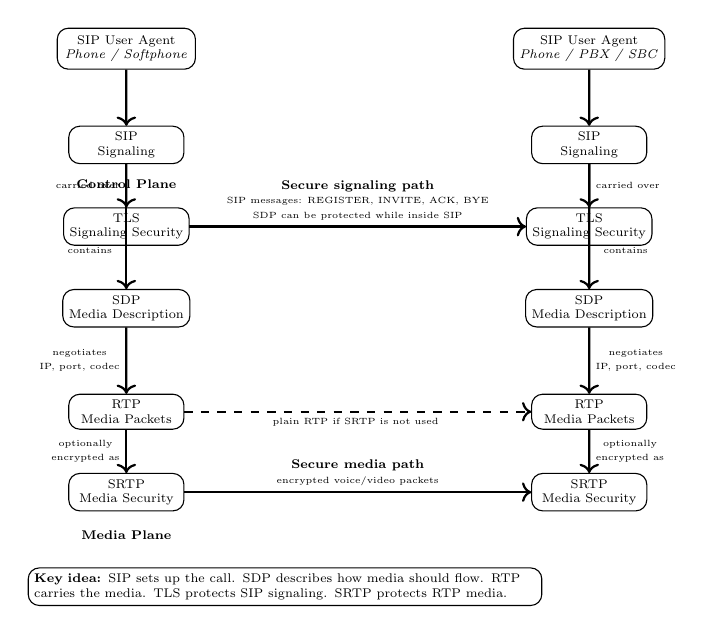
\begin{tikzpicture}[
    scale=0.65,
    transform shape,
    font=\scriptsize,
    node distance=1.25cm,
    box/.style={
        rectangle,
        rounded corners,
        draw,
        align=center,
        minimum width=2.7cm,
        minimum height=0.8cm
    },
    smallbox/.style={
        rectangle,
        rounded corners,
        draw,
        align=center,
        minimum width=2.25cm,
        minimum height=0.65cm
    },
    arrow/.style={->, thick},
    dashedarrow/.style={->, thick, dashed}
]

% Endpoints
\node[box] (ua1) {SIP User Agent\\\textit{Phone / Softphone}};
\node[box, right=6.2cm of ua1] (ua2) {SIP User Agent\\\textit{Phone / PBX / SBC}};

% Signaling layer
\node[smallbox, below=1.1cm of ua1] (sip1) {SIP\\Signaling};
\node[smallbox, below=1.1cm of ua2] (sip2) {SIP\\Signaling};

\node[smallbox, below=0.85cm of sip1] (tls1) {TLS\\Signaling Security};
\node[smallbox, below=0.85cm of sip2] (tls2) {TLS\\Signaling Security};

% SDP body
\node[smallbox, below=0.85cm of tls1] (sdp1) {SDP\\Media Description};
\node[smallbox, below=0.85cm of tls2] (sdp2) {SDP\\Media Description};

% Media layer
\node[smallbox, below=1.3cm of sdp1] (rtp1) {RTP\\Media Packets};
\node[smallbox, below=1.3cm of sdp2] (rtp2) {RTP\\Media Packets};

\node[smallbox, below=0.85cm of rtp1] (srtp1) {SRTP\\Media Security};
\node[smallbox, below=0.85cm of rtp2] (srtp2) {SRTP\\Media Security};

% Internal vertical relationships
\draw[arrow] (ua1) -- (sip1);
\draw[arrow] (ua2) -- (sip2);

\draw[arrow] (sip1) -- node[left, align=center] {\tiny carried over} (tls1);
\draw[arrow] (sip2) -- node[right, align=center] {\tiny carried over} (tls2);

\draw[arrow] (sip1) -- node[above left, xshift=-0.15cm, yshift=-0.65cm] {\tiny contains} (sdp1);
\draw[arrow] (sip2) -- node[above right, xshift=0.15cm, yshift=-0.65cm] {\tiny contains} (sdp2);

\draw[arrow] (sdp1) -- node[left, align=center] {\tiny negotiates\\\tiny IP, port, codec} (rtp1);
\draw[arrow] (sdp2) -- node[right, align=center] {\tiny negotiates\\\tiny IP, port, codec} (rtp2);

\draw[arrow] (rtp1) -- node[left, align=center] {\tiny optionally\\\tiny encrypted as} (srtp1);
\draw[arrow] (rtp2) -- node[right, align=center] {\tiny optionally\\\tiny encrypted as} (srtp2);

% Cross-system flows
\draw[arrow] (tls1.east) -- node[above, align=center] {
    \textbf{Secure signaling path}\\
    \tiny SIP messages: REGISTER, INVITE, ACK, BYE\\
    \tiny SDP can be protected while inside SIP
} (tls2.west);

\draw[arrow] (srtp1.east) -- node[above, align=center] {
    \textbf{Secure media path}\\
    \tiny encrypted voice/video packets
} (srtp2.west);

\draw[dashedarrow] (rtp1.east) -- node[below, align=center] {
    \tiny plain RTP if SRTP is not used
} (rtp2.west);

% Labels
\node[align=center, above=0.25cm of tls1] {\textbf{Control Plane}};
\node[align=center, below=0.25cm of srtp1] {\textbf{Media Plane}};

% Key idea box
\node[
    rectangle,
    rounded corners,
    draw,
    align=left,
    text width=9.8cm,
    below=1.1cm of srtp1,
    xshift=3.1cm
] (keyidea) {
    \textbf{Key idea:}
    SIP sets up the call. SDP describes how media should flow.
    RTP carries the media. TLS protects SIP signaling.
    SRTP protects RTP media.
};

\end{tikzpicture}

\end{frame}


\begin{frame}{Common SIP Headers: Routing and Dialog Identity}
\scriptsize
\begin{tabular}{p{2.4cm} p{4.5cm} p{5.2cm}}
\toprule
\textbf{Header} & \textbf{Purpose} & \textbf{Example / Meaning} \\
\midrule
\texttt{Via} & Records each SIP hop so responses can route back & \texttt{Via: SIP/2.0/UDP proxy.local;branch=z9hG4bK1} \\
\texttt{Route} & Forces a request through listed proxies & Used after \texttt{Record-Route} keeps a proxy in path \\
\texttt{Record-Route} & Tells endpoints to keep this proxy in future dialog messages & Common for SBCs/proxies that must stay involved \\
\texttt{Max-Forwards} & Prevents endless proxy loops & Usually starts at \texttt{70}; decremented per hop \\
\texttt{From} & Logical identity of caller & \texttt{From: <sip:6001@pbx.local>;tag=abc123} \\
\texttt{To} & Logical identity of callee & \texttt{To: <sip:6002@pbx.local>;tag=xyz789} \\
\texttt{Call-ID} & Globally identifies a call/dialog & Same across messages in the same dialog \\
\texttt{CSeq} & Orders requests within a dialog & \texttt{CSeq: 1 INVITE}, then \texttt{CSeq: 2 BYE} \\
\texttt{Contact} & Direct address for future requests & NAT issues often involve bad \texttt{Contact} values \\
\texttt{Request-URI} & Target of the SIP request & \texttt{INVITE sip:6002@pbx.local SIP/2.0} \\
\bottomrule
\end{tabular}

\vspace{0.2cm}
\begin{block}{Key idea}
Headers like \texttt{Via}, \texttt{Route}, \texttt{Contact}, \texttt{Call-ID}, and tags are how SIP tracks where messages go and which call/dialog they belong to.
\end{block}
\end{frame}


\begin{frame}{Common SIP Headers: Capabilities, Auth, and Message Body}
\scriptsize
\begin{tabular}{p{2.7cm} p{4.4cm} p{5.0cm}}
\toprule
\textbf{Header} & \textbf{Purpose} & \textbf{Example / Meaning} \\
\midrule
\texttt{Content-Type} & Describes SIP message body & \texttt{Content-Type: application/sdp} \\
\texttt{Content-Length} & Body size in bytes & Important for parsing SIP over TCP/TLS \\
\texttt{Allow} & Lists supported SIP methods & \texttt{Allow: INVITE, ACK, BYE, CANCEL, OPTIONS} \\
\texttt{Supported} & Lists optional SIP extensions supported & \texttt{Supported: replaces, timer, 100rel} \\
\texttt{Require} & Demands support for an extension & If unsupported, receiver may reject request \\
\texttt{User-Agent} & Identifies endpoint software/device & \texttt{User-Agent: Asterisk PBX} \\
\texttt{Server} & Identifies server software & Often hidden by SBCs for security \\
\texttt{Authorization} & Digest credentials from client & Used after \texttt{401 Unauthorized} challenge \\
\texttt{Proxy-Authorization} & Digest credentials for proxy/auth server & Used after \texttt{407 Proxy Authentication Required} \\
\texttt{WWW-Authenticate} & Server auth challenge & Contains realm, nonce, algorithm \\
\texttt{Proxy-Authenticate} & Proxy auth challenge & Similar to \texttt{WWW-Authenticate} \\
\texttt{Expires} & Registration/contact lifetime & \texttt{Expires: 3600} means register for 1 hour \\
\texttt{P-Asserted-Identity} & Trusted caller identity inside provider networks & Common in carrier/SBC environments \\
\bottomrule
\end{tabular}
\end{frame}

\begin{frame}{Key idea}
\begin{block}{Key idea}
Headers like \texttt{Content-Type}, \texttt{Authorization}, \texttt{Supported}, and \texttt{Expires} tell SIP peers how to parse, authenticate, and negotiate behavior.
\end{block}
\end{frame}


\begin{frame}{The 10 Commandments of SIP, SDP, RTP, SRTP, and TLS}
\scriptsize

\begin{enumerate}
    \item \textbf{SIP is the control plane.}  
    It sets up, modifies, and tears down sessions. It does not carry the voice or video.

    \item \textbf{SDP is the media contract.}  
    It lives inside SIP messages and describes codec, media type, IP address, port, and direction.

    \item \textbf{RTP is the media plane.}  
    It carries the actual real-time audio or video packets after SIP and SDP negotiation.

    \item \textbf{TLS protects SIP signaling.}  
    SIP over TLS encrypts call setup messages such as \texttt{REGISTER}, \texttt{INVITE}, \texttt{ACK}, and \texttt{BYE}.

    \item \textbf{SRTP protects RTP media.}  
    TLS does not encrypt the voice stream by itself. Use SRTP when the audio or video must be protected.

    \item \textbf{A successful SIP call does not guarantee working audio.}  
    SIP can complete while RTP fails because signaling and media often take different network paths.

    \item \textbf{Bad SDP often causes one-way or no audio.}  
    If SDP advertises the wrong IP address, private IP, blocked port, or unsupported codec, media can break.

    \item \textbf{NAT and firewalls are usually media problems.}  
    Many ``SIP problems'' are really RTP reachability problems caused by blocked UDP ports or bad address translation.

    \item \textbf{SIP headers identify, route, and track the call.}  
    \texttt{Via}, \texttt{Contact}, \texttt{From}, \texttt{To}, \texttt{Call-ID}, and \texttt{CSeq} tell SIP where messages go and which dialog they belong to.

    \item \textbf{Always debug in layers.}  
    First check registration, then SIP call flow, then SDP negotiation, then RTP/SRTP packet flow, then TLS/security settings.
\end{enumerate}

\vspace{0.15cm}

\begin{block}{Mental model}
\centering
\texttt{SIP + TLS = secure signaling}
\quad
\texttt{SDP = media instructions}
\quad
\texttt{RTP + SRTP = secure media}
\end{block}

\end{frame}





\begin{frame}{The Same Call Seen Two Ways}
\scriptsize
\centering

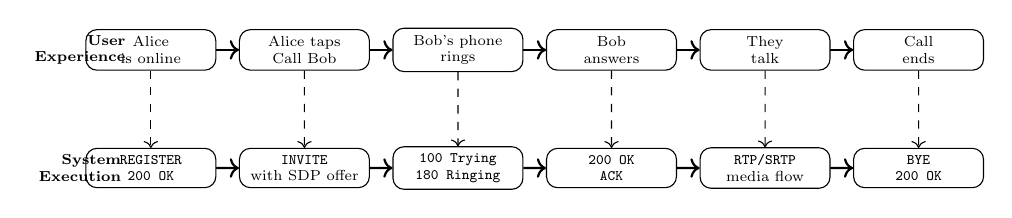
\begin{tikzpicture}[
    scale=0.75,
    transform shape,
    font=\scriptsize,
    event/.style={
        rectangle,
        rounded corners,
        draw,
        align=center,
        minimum width=2.2cm,
        minimum height=0.65cm
    },
    proto/.style={
        rectangle,
        rounded corners,
        draw,
        align=center,
        minimum width=2.2cm,
        minimum height=0.65cm
    },
    arrow/.style={->, thick}
]

% Timeline labels
\node[align=right] at (-1.2,0) {\textbf{User}\\\textbf{Experience}};
\node[align=right] at (-1.2,-2.0) {\textbf{System}\\\textbf{Execution}};

% User experience row
\node[event] (u1) at (0,0) {Alice\\is online};
\node[event] (u2) at (2.6,0) {Alice taps\\Call Bob};
\node[event] (u3) at (5.2,0) {Bob's phone\\rings};
\node[event] (u4) at (7.8,0) {Bob\\answers};
\node[event] (u5) at (10.4,0) {They\\talk};
\node[event] (u6) at (13.0,0) {Call\\ends};

% System execution row
\node[proto] (p1) at (0,-2.0) {\texttt{REGISTER}\\\texttt{200 OK}};
\node[proto] (p2) at (2.6,-2.0) {\texttt{INVITE}\\with SDP offer};
\node[proto] (p3) at (5.2,-2.0) {\texttt{100 Trying}\\\texttt{180 Ringing}};
\node[proto] (p4) at (7.8,-2.0) {\texttt{200 OK}\\\texttt{ACK}};
\node[proto] (p5) at (10.4,-2.0) {\texttt{RTP/SRTP}\\media flow};
\node[proto] (p6) at (13.0,-2.0) {\texttt{BYE}\\\texttt{200 OK}};

% Horizontal arrows user row
\draw[arrow] (u1) -- (u2);
\draw[arrow] (u2) -- (u3);
\draw[arrow] (u3) -- (u4);
\draw[arrow] (u4) -- (u5);
\draw[arrow] (u5) -- (u6);

% Horizontal arrows protocol row
\draw[arrow] (p1) -- (p2);
\draw[arrow] (p2) -- (p3);
\draw[arrow] (p3) -- (p4);
\draw[arrow] (p4) -- (p5);
\draw[arrow] (p5) -- (p6);

% Mapping arrows
\draw[dashed, ->] (u1) -- (p1);
\draw[dashed, ->] (u2) -- (p2);
\draw[dashed, ->] (u3) -- (p3);
\draw[dashed, ->] (u4) -- (p4);
\draw[dashed, ->] (u5) -- (p5);
\draw[dashed, ->] (u6) -- (p6);

\end{tikzpicture}

\vspace{0.3cm}

\begin{block}{Key idea}
SIP makes the call experience possible, SDP tells media where/how to flow, RTP/SRTP carries the actual conversation, and TLS can protect the signaling.
\end{block}

\end{frame}


\begin{frame}{Why SIP Security Is Worth Learning Deeply}
\tiny

\begin{block}{The real system is not ``a phone call.''}
A secure VoIP session is a distributed protocol stack that combines identity, routing,
cryptographic keying, media negotiation, NAT traversal, and real-time packet delivery.
\end{block}

\vspace{0.1cm}

\begin{columns}[T]
\column{0.48\textwidth}

\textbf{Signaling plane}

\vspace{0.05cm}

\begin{itemize}
    \item \textbf{SIP} establishes dialog state using \texttt{Call-ID}, \texttt{From/To} tags, \texttt{CSeq}, \texttt{Via}, \texttt{Contact}, and \texttt{Route}.
    \item \textbf{Digest auth} proves endpoint knowledge of a shared secret without sending the password directly.
    \item \textbf{TLS} protects SIP messages in transit:
    \begin{itemize}
        \tiny
        \item confidentiality
        \item integrity
        \item server authentication
        \item optional mutual authentication
    \end{itemize}
    \item \textbf{SDP} inside SIP describes the media offer/answer:
    \begin{itemize}
        \tiny
        \item codec
        \item RTP port
        \item IP address
        \item media direction
        \item SRTP crypto parameters
    \end{itemize}
\end{itemize}

\column{0.48\textwidth}

\textbf{Media plane}

\vspace{0.05cm}

\begin{itemize}
    \item \textbf{RTP} carries real-time voice/video with sequence numbers, timestamps, payload types, and SSRCs.
    \item \textbf{RTCP} reports media quality:
    \begin{itemize}
        \tiny
        \item packet loss
        \item jitter
        \item sender/receiver timing
        \item round-trip estimates
    \end{itemize}
    \item \textbf{SRTP} adds media protection:
    \begin{itemize}
        \tiny
        \item encryption
        \item authentication
        \item replay protection
        \item packet-index based keystream generation
    \end{itemize}
    \item \textbf{NAT/firewalls} force engineering decisions:
    \begin{itemize}
        \tiny
        \item symmetric RTP
        \item media anchoring
        \item SBCs
        \item ICE/STUN/TURN in WebRTC-style systems
    \end{itemize}
\end{itemize}

\end{columns}

\end{frame}

\begin{frame}{Challenge}

\begin{alertblock}{The engineering challenge}
\centering
SIP/TLS may prove who is allowed to set up the session, but RTP/SRTP determines whether the real-time conversation actually arrives, stays private, and remains usable under loss, jitter, NAT, and attack.
\end{alertblock}

\end{frame}


\end{document}
